% Created by tikzDevice version 0.12.3.1 on 2023-10-23 15:56:17
% !TEX encoding = UTF-8 Unicode
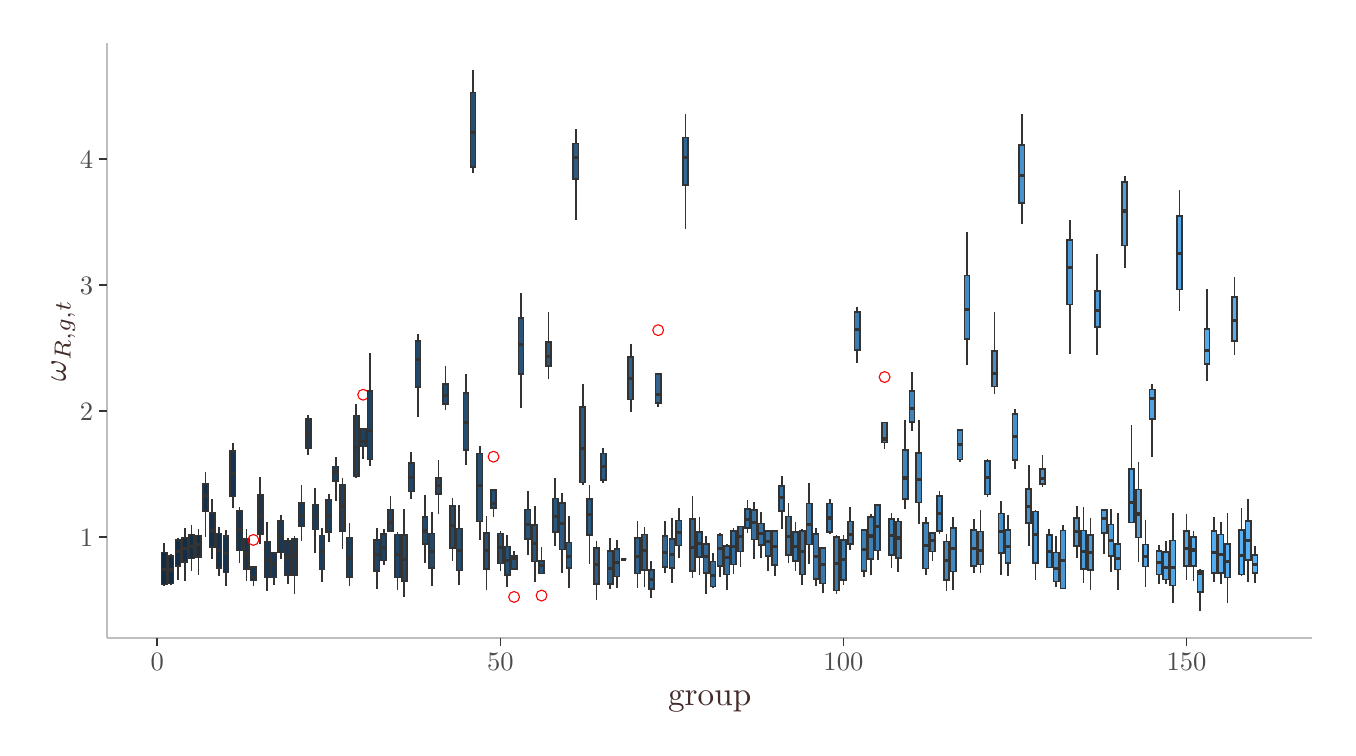
\begin{tikzpicture}[x=1pt,y=1pt]
\definecolor{fillColor}{RGB}{255,255,255}
\path[use as bounding box,fill=fillColor,fill opacity=0.00] (0,0) rectangle (469.75,252.94);
\begin{scope}
\path[clip] (  0.00,  0.00) rectangle (469.75,252.94);
\definecolor{drawColor}{RGB}{255,255,255}
\definecolor{fillColor}{RGB}{255,255,255}

\path[draw=drawColor,line width= 0.6pt,line join=round,line cap=round,fill=fillColor] (  0.00,  0.00) rectangle (469.76,252.94);
\end{scope}
\begin{scope}
\path[clip] ( 28.60, 32.28) rectangle (464.25,247.44);
\definecolor{drawColor}{RGB}{255,255,255}

\path[draw=drawColor,line width= 0.6pt,line join=round] ( 28.60, 68.78) --
	(464.25, 68.78);

\path[draw=drawColor,line width= 0.6pt,line join=round] ( 28.60,114.35) --
	(464.25,114.35);

\path[draw=drawColor,line width= 0.6pt,line join=round] ( 28.60,159.93) --
	(464.25,159.93);

\path[draw=drawColor,line width= 0.6pt,line join=round] ( 28.60,205.51) --
	(464.25,205.51);

\path[draw=drawColor,line width= 0.6pt,line join=round] ( 46.85, 32.28) --
	( 46.85,247.44);

\path[draw=drawColor,line width= 0.6pt,line join=round] (170.81, 32.28) --
	(170.81,247.44);

\path[draw=drawColor,line width= 0.6pt,line join=round] (294.77, 32.28) --
	(294.77,247.44);

\path[draw=drawColor,line width= 0.6pt,line join=round] (418.73, 32.28) --
	(418.73,247.44);
\definecolor{drawColor}{gray}{0.20}

\path[draw=drawColor,line width= 0.6pt,line join=round] ( 49.33, 63.31) -- ( 49.33, 66.76);

\path[draw=drawColor,line width= 0.6pt,line join=round] ( 49.33, 51.72) -- ( 49.33, 51.31);
\definecolor{fillColor}{RGB}{19,43,67}

\path[draw=drawColor,line width= 0.6pt,fill=fillColor] ( 48.40, 63.31) --
	( 48.40, 51.72) --
	( 50.26, 51.72) --
	( 50.26, 63.31) --
	( 48.40, 63.31) --
	cycle;

\path[draw=drawColor,line width= 1.1pt] ( 48.40, 57.01) -- ( 50.26, 57.01);

\path[draw=drawColor,line width= 0.6pt,line join=round] ( 51.81, 62.06) -- ( 51.81, 62.68);

\path[draw=drawColor,line width= 0.6pt,line join=round] ( 51.81, 52.08) -- ( 51.81, 52.07);
\definecolor{fillColor}{RGB}{19,44,68}

\path[draw=drawColor,line width= 0.6pt,fill=fillColor] ( 50.88, 62.06) --
	( 50.88, 52.08) --
	( 52.74, 52.08) --
	( 52.74, 62.06) --
	( 50.88, 62.06) --
	cycle;

\path[draw=drawColor,line width= 1.1pt] ( 50.88, 56.97) -- ( 52.74, 56.97);

\path[draw=drawColor,line width= 0.6pt,line join=round] ( 54.29, 67.76) -- ( 54.29, 68.60);

\path[draw=drawColor,line width= 0.6pt,line join=round] ( 54.29, 58.32) -- ( 54.29, 53.37);
\definecolor{fillColor}{RGB}{20,44,69}

\path[draw=drawColor,line width= 0.6pt,fill=fillColor] ( 53.36, 67.76) --
	( 53.36, 58.32) --
	( 55.22, 58.32) --
	( 55.22, 67.76) --
	( 53.36, 67.76) --
	cycle;

\path[draw=drawColor,line width= 1.1pt] ( 53.36, 63.73) -- ( 55.22, 63.73);

\path[draw=drawColor,line width= 0.6pt,line join=round] ( 56.77, 68.45) -- ( 56.77, 72.10);

\path[draw=drawColor,line width= 0.6pt,line join=round] ( 56.77, 59.86) -- ( 56.77, 53.17);
\definecolor{fillColor}{RGB}{20,45,70}

\path[draw=drawColor,line width= 0.6pt,fill=fillColor] ( 55.84, 68.45) --
	( 55.84, 59.86) --
	( 57.70, 59.86) --
	( 57.70, 68.45) --
	( 55.84, 68.45) --
	cycle;

\path[draw=drawColor,line width= 1.1pt] ( 55.84, 64.66) -- ( 57.70, 64.66);

\path[draw=drawColor,line width= 0.6pt,line join=round] ( 59.25, 69.75) -- ( 59.25, 73.17);

\path[draw=drawColor,line width= 0.6pt,line join=round] ( 59.25, 61.08) -- ( 59.25, 56.76);
\definecolor{fillColor}{RGB}{20,46,71}

\path[draw=drawColor,line width= 0.6pt,fill=fillColor] ( 58.32, 69.75) --
	( 58.32, 61.08) --
	( 60.18, 61.08) --
	( 60.18, 69.75) --
	( 58.32, 69.75) --
	cycle;

\path[draw=drawColor,line width= 1.1pt] ( 58.32, 65.57) -- ( 60.18, 65.57);

\path[draw=drawColor,line width= 0.6pt,line join=round] ( 61.72, 69.42) -- ( 61.72, 71.77);

\path[draw=drawColor,line width= 0.6pt,line join=round] ( 61.72, 61.60) -- ( 61.72, 55.08);
\definecolor{fillColor}{RGB}{21,47,72}

\path[draw=drawColor,line width= 0.6pt,fill=fillColor] ( 60.79, 69.42) --
	( 60.79, 61.60) --
	( 62.65, 61.60) --
	( 62.65, 69.42) --
	( 60.79, 69.42) --
	cycle;

\path[draw=drawColor,line width= 1.1pt] ( 60.79, 66.20) -- ( 62.65, 66.20);

\path[draw=drawColor,line width= 0.6pt,line join=round] ( 64.20, 87.93) -- ( 64.20, 92.50);

\path[draw=drawColor,line width= 0.6pt,line join=round] ( 64.20, 78.33) -- ( 64.20, 68.97);
\definecolor{fillColor}{RGB}{21,47,73}

\path[draw=drawColor,line width= 0.6pt,fill=fillColor] ( 63.27, 87.93) --
	( 63.27, 78.33) --
	( 65.13, 78.33) --
	( 65.13, 87.93) --
	( 63.27, 87.93) --
	cycle;

\path[draw=drawColor,line width= 1.1pt] ( 63.27, 83.93) -- ( 65.13, 83.93);

\path[draw=drawColor,line width= 0.6pt,line join=round] ( 66.68, 77.57) -- ( 66.68, 82.47);

\path[draw=drawColor,line width= 0.6pt,line join=round] ( 66.68, 65.30) -- ( 66.68, 60.79);
\definecolor{fillColor}{RGB}{22,48,74}

\path[draw=drawColor,line width= 0.6pt,fill=fillColor] ( 65.75, 77.57) --
	( 65.75, 65.30) --
	( 67.61, 65.30) --
	( 67.61, 77.57) --
	( 65.75, 77.57) --
	cycle;

\path[draw=drawColor,line width= 1.1pt] ( 65.75, 71.37) -- ( 67.61, 71.37);

\path[draw=drawColor,line width= 0.6pt,line join=round] ( 69.16, 70.17) -- ( 69.16, 72.48);

\path[draw=drawColor,line width= 0.6pt,line join=round] ( 69.16, 57.70) -- ( 69.16, 54.89);
\definecolor{fillColor}{RGB}{22,49,75}

\path[draw=drawColor,line width= 0.6pt,fill=fillColor] ( 68.23, 70.17) --
	( 68.23, 57.70) --
	( 70.09, 57.70) --
	( 70.09, 70.17) --
	( 68.23, 70.17) --
	cycle;

\path[draw=drawColor,line width= 1.1pt] ( 68.23, 64.02) -- ( 70.09, 64.02);

\path[draw=drawColor,line width= 0.6pt,line join=round] ( 71.64, 69.25) -- ( 71.64, 71.46);

\path[draw=drawColor,line width= 0.6pt,line join=round] ( 71.64, 56.09) -- ( 71.64, 51.27);
\definecolor{fillColor}{RGB}{22,50,76}

\path[draw=drawColor,line width= 0.6pt,fill=fillColor] ( 70.71, 69.25) --
	( 70.71, 56.09) --
	( 72.57, 56.09) --
	( 72.57, 69.25) --
	( 70.71, 69.25) --
	cycle;

\path[draw=drawColor,line width= 1.1pt] ( 70.71, 63.10) -- ( 72.57, 63.10);

\path[draw=drawColor,line width= 0.6pt,line join=round] ( 74.12, 99.91) -- ( 74.12,102.91);

\path[draw=drawColor,line width= 0.6pt,line join=round] ( 74.12, 83.55) -- ( 74.12, 79.21);
\definecolor{fillColor}{RGB}{23,50,77}

\path[draw=drawColor,line width= 0.6pt,fill=fillColor] ( 73.19, 99.91) --
	( 73.19, 83.55) --
	( 75.05, 83.55) --
	( 75.05, 99.91) --
	( 73.19, 99.91) --
	cycle;

\path[draw=drawColor,line width= 1.1pt] ( 73.19, 91.96) -- ( 75.05, 91.96);

\path[draw=drawColor,line width= 0.6pt,line join=round] ( 76.60, 78.25) -- ( 76.60, 79.59);

\path[draw=drawColor,line width= 0.6pt,line join=round] ( 76.60, 63.99) -- ( 76.60, 59.42);
\definecolor{fillColor}{RGB}{23,51,78}

\path[draw=drawColor,line width= 0.6pt,fill=fillColor] ( 75.67, 78.25) --
	( 75.67, 63.99) --
	( 77.53, 63.99) --
	( 77.53, 78.25) --
	( 75.67, 78.25) --
	cycle;

\path[draw=drawColor,line width= 1.1pt] ( 75.67, 71.66) -- ( 77.53, 71.66);

\path[draw=drawColor,line width= 0.6pt,line join=round] ( 79.08, 68.41) -- ( 79.08, 71.70);

\path[draw=drawColor,line width= 0.6pt,line join=round] ( 79.08, 57.38) -- ( 79.08, 52.83);
\definecolor{fillColor}{RGB}{24,52,79}

\path[draw=drawColor,line width= 0.6pt,fill=fillColor] ( 78.15, 68.41) --
	( 78.15, 57.38) --
	( 80.01, 57.38) --
	( 80.01, 68.41) --
	( 78.15, 68.41) --
	cycle;

\path[draw=drawColor,line width= 1.1pt] ( 78.15, 63.10) -- ( 80.01, 63.10);
\definecolor{drawColor}{RGB}{255,0,0}

\path[draw=drawColor,line width= 0.4pt,line join=round,line cap=round] ( 81.56, 67.84) circle (  1.96);
\definecolor{drawColor}{gray}{0.20}

\path[draw=drawColor,line width= 0.6pt,line join=round] ( 81.56, 58.14) -- ( 81.56, 58.14);

\path[draw=drawColor,line width= 0.6pt,line join=round] ( 81.56, 53.22) -- ( 81.56, 51.02);
\definecolor{fillColor}{RGB}{24,53,80}

\path[draw=drawColor,line width= 0.6pt,fill=fillColor] ( 80.63, 58.14) --
	( 80.63, 53.22) --
	( 82.49, 53.22) --
	( 82.49, 58.14) --
	( 80.63, 58.14) --
	cycle;

\path[draw=drawColor,line width= 1.1pt] ( 80.63, 54.43) -- ( 82.49, 54.43);

\path[draw=drawColor,line width= 0.6pt,line join=round] ( 84.04, 84.23) -- ( 84.04, 90.49);

\path[draw=drawColor,line width= 0.6pt,line join=round] ( 84.04, 69.95) -- ( 84.04, 66.51);
\definecolor{fillColor}{RGB}{24,53,81}

\path[draw=drawColor,line width= 0.6pt,fill=fillColor] ( 83.11, 84.23) --
	( 83.11, 69.95) --
	( 84.97, 69.95) --
	( 84.97, 84.23) --
	( 83.11, 84.23) --
	cycle;

\path[draw=drawColor,line width= 1.1pt] ( 83.11, 76.62) -- ( 84.97, 76.62);

\path[draw=drawColor,line width= 0.6pt,line join=round] ( 86.52, 67.23) -- ( 86.52, 74.14);

\path[draw=drawColor,line width= 0.6pt,line join=round] ( 86.52, 54.28) -- ( 86.52, 49.52);
\definecolor{fillColor}{RGB}{25,54,82}

\path[draw=drawColor,line width= 0.6pt,fill=fillColor] ( 85.59, 67.23) --
	( 85.59, 54.28) --
	( 87.45, 54.28) --
	( 87.45, 67.23) --
	( 85.59, 67.23) --
	cycle;

\path[draw=drawColor,line width= 1.1pt] ( 85.59, 60.40) -- ( 87.45, 60.40);

\path[draw=drawColor,line width= 0.6pt,line join=round] ( 89.00, 63.12) -- ( 89.00, 63.34);

\path[draw=drawColor,line width= 0.6pt,line join=round] ( 89.00, 54.21) -- ( 89.00, 51.47);
\definecolor{fillColor}{RGB}{25,55,83}

\path[draw=drawColor,line width= 0.6pt,fill=fillColor] ( 88.07, 63.12) --
	( 88.07, 54.21) --
	( 89.93, 54.21) --
	( 89.93, 63.12) --
	( 88.07, 63.12) --
	cycle;

\path[draw=drawColor,line width= 1.1pt] ( 88.07, 59.08) -- ( 89.93, 59.08);

\path[draw=drawColor,line width= 0.6pt,line join=round] ( 91.48, 74.67) -- ( 91.48, 76.76);

\path[draw=drawColor,line width= 0.6pt,line join=round] ( 91.48, 63.45) -- ( 91.48, 60.90);
\definecolor{fillColor}{RGB}{25,56,84}

\path[draw=drawColor,line width= 0.6pt,fill=fillColor] ( 90.55, 74.67) --
	( 90.55, 63.45) --
	( 92.40, 63.45) --
	( 92.40, 74.67) --
	( 90.55, 74.67) --
	cycle;

\path[draw=drawColor,line width= 1.1pt] ( 90.55, 69.14) -- ( 92.40, 69.14);

\path[draw=drawColor,line width= 0.6pt,line join=round] ( 93.95, 67.34) -- ( 93.95, 68.56);

\path[draw=drawColor,line width= 0.6pt,line join=round] ( 93.95, 55.24) -- ( 93.95, 51.81);
\definecolor{fillColor}{RGB}{26,56,85}

\path[draw=drawColor,line width= 0.6pt,fill=fillColor] ( 93.02, 67.34) --
	( 93.02, 55.24) --
	( 94.88, 55.24) --
	( 94.88, 67.34) --
	( 93.02, 67.34) --
	cycle;

\path[draw=drawColor,line width= 1.1pt] ( 93.02, 61.66) -- ( 94.88, 61.66);

\path[draw=drawColor,line width= 0.6pt,line join=round] ( 96.43, 68.29) -- ( 96.43, 69.28);

\path[draw=drawColor,line width= 0.6pt,line join=round] ( 96.43, 55.12) -- ( 96.43, 48.12);
\definecolor{fillColor}{RGB}{26,57,86}

\path[draw=drawColor,line width= 0.6pt,fill=fillColor] ( 95.50, 68.29) --
	( 95.50, 55.12) --
	( 97.36, 55.12) --
	( 97.36, 68.29) --
	( 95.50, 68.29) --
	cycle;

\path[draw=drawColor,line width= 1.1pt] ( 95.50, 62.70) -- ( 97.36, 62.70);

\path[draw=drawColor,line width= 0.6pt,line join=round] ( 98.91, 81.07) -- ( 98.91, 87.72);

\path[draw=drawColor,line width= 0.6pt,line join=round] ( 98.91, 72.74) -- ( 98.91, 67.49);
\definecolor{fillColor}{RGB}{27,58,87}

\path[draw=drawColor,line width= 0.6pt,fill=fillColor] ( 97.98, 81.07) --
	( 97.98, 72.74) --
	( 99.84, 72.74) --
	( 99.84, 81.07) --
	( 97.98, 81.07) --
	cycle;

\path[draw=drawColor,line width= 1.1pt] ( 97.98, 76.67) -- ( 99.84, 76.67);

\path[draw=drawColor,line width= 0.6pt,line join=round] (101.39,111.52) -- (101.39,112.96);

\path[draw=drawColor,line width= 0.6pt,line join=round] (101.39,100.85) -- (101.39, 98.65);
\definecolor{fillColor}{RGB}{27,59,88}

\path[draw=drawColor,line width= 0.6pt,fill=fillColor] (100.46,111.52) --
	(100.46,100.85) --
	(102.32,100.85) --
	(102.32,111.52) --
	(100.46,111.52) --
	cycle;

\path[draw=drawColor,line width= 1.1pt] (100.46,106.31) -- (102.32,106.31);

\path[draw=drawColor,line width= 0.6pt,line join=round] (103.87, 80.50) -- (103.87, 86.54);

\path[draw=drawColor,line width= 0.6pt,line join=round] (103.87, 71.56) -- (103.87, 63.04);
\definecolor{fillColor}{RGB}{27,60,89}

\path[draw=drawColor,line width= 0.6pt,fill=fillColor] (102.94, 80.50) --
	(102.94, 71.56) --
	(104.80, 71.56) --
	(104.80, 80.50) --
	(102.94, 80.50) --
	cycle;

\path[draw=drawColor,line width= 1.1pt] (102.94, 76.45) -- (104.80, 76.45);

\path[draw=drawColor,line width= 0.6pt,line join=round] (106.35, 69.47) -- (106.35, 72.21);

\path[draw=drawColor,line width= 0.6pt,line join=round] (106.35, 57.12) -- (106.35, 52.79);
\definecolor{fillColor}{RGB}{28,60,90}

\path[draw=drawColor,line width= 0.6pt,fill=fillColor] (105.42, 69.47) --
	(105.42, 57.12) --
	(107.28, 57.12) --
	(107.28, 69.47) --
	(105.42, 69.47) --
	cycle;

\path[draw=drawColor,line width= 1.1pt] (105.42, 63.56) -- (107.28, 63.56);

\path[draw=drawColor,line width= 0.6pt,line join=round] (108.83, 82.40) -- (108.83, 84.37);

\path[draw=drawColor,line width= 0.6pt,line join=round] (108.83, 70.68) -- (108.83, 66.94);
\definecolor{fillColor}{RGB}{28,61,91}

\path[draw=drawColor,line width= 0.6pt,fill=fillColor] (107.90, 82.40) --
	(107.90, 70.68) --
	(109.76, 70.68) --
	(109.76, 82.40) --
	(107.90, 82.40) --
	cycle;

\path[draw=drawColor,line width= 1.1pt] (107.90, 76.83) -- (109.76, 76.83);

\path[draw=drawColor,line width= 0.6pt,line join=round] (111.31, 94.39) -- (111.31, 97.97);

\path[draw=drawColor,line width= 0.6pt,line join=round] (111.31, 89.17) -- (111.31, 81.94);
\definecolor{fillColor}{RGB}{29,62,92}

\path[draw=drawColor,line width= 0.6pt,fill=fillColor] (110.38, 94.39) --
	(110.38, 89.17) --
	(112.24, 89.17) --
	(112.24, 94.39) --
	(110.38, 94.39) --
	cycle;

\path[draw=drawColor,line width= 1.1pt] (110.38, 92.38) -- (112.24, 92.38);

\path[draw=drawColor,line width= 0.6pt,line join=round] (113.79, 87.73) -- (113.79, 90.14);

\path[draw=drawColor,line width= 0.6pt,line join=round] (113.79, 71.04) -- (113.79, 64.53);
\definecolor{fillColor}{RGB}{29,63,93}

\path[draw=drawColor,line width= 0.6pt,fill=fillColor] (112.86, 87.73) --
	(112.86, 71.04) --
	(114.72, 71.04) --
	(114.72, 87.73) --
	(112.86, 87.73) --
	cycle;

\path[draw=drawColor,line width= 1.1pt] (112.86, 80.07) -- (114.72, 80.07);

\path[draw=drawColor,line width= 0.6pt,line join=round] (116.27, 68.74) -- (116.27, 73.86);

\path[draw=drawColor,line width= 0.6pt,line join=round] (116.27, 54.46) -- (116.27, 51.09);
\definecolor{fillColor}{RGB}{29,63,94}

\path[draw=drawColor,line width= 0.6pt,fill=fillColor] (115.34, 68.74) --
	(115.34, 54.46) --
	(117.20, 54.46) --
	(117.20, 68.74) --
	(115.34, 68.74) --
	cycle;

\path[draw=drawColor,line width= 1.1pt] (115.34, 61.31) -- (117.20, 61.31);

\path[draw=drawColor,line width= 0.6pt,line join=round] (118.75,112.81) -- (118.75,116.93);

\path[draw=drawColor,line width= 0.6pt,line join=round] (118.75, 91.03) -- (118.75, 90.27);
\definecolor{fillColor}{RGB}{30,64,96}

\path[draw=drawColor,line width= 0.6pt,fill=fillColor] (117.82,112.81) --
	(117.82, 91.03) --
	(119.68, 91.03) --
	(119.68,112.81) --
	(117.82,112.81) --
	cycle;

\path[draw=drawColor,line width= 1.1pt] (117.82,101.36) -- (119.68,101.36);
\definecolor{drawColor}{RGB}{255,0,0}

\path[draw=drawColor,line width= 0.4pt,line join=round,line cap=round] (121.23,120.30) circle (  1.96);
\definecolor{drawColor}{gray}{0.20}

\path[draw=drawColor,line width= 0.6pt,line join=round] (121.23,107.84) -- (121.23,107.84);

\path[draw=drawColor,line width= 0.6pt,line join=round] (121.23,101.64) -- (121.23, 97.15);
\definecolor{fillColor}{RGB}{30,65,97}

\path[draw=drawColor,line width= 0.6pt,fill=fillColor] (120.30,107.84) --
	(120.30,101.64) --
	(122.16,101.64) --
	(122.16,107.84) --
	(120.30,107.84) --
	cycle;

\path[draw=drawColor,line width= 1.1pt] (120.30,103.41) -- (122.16,103.41);

\path[draw=drawColor,line width= 0.6pt,line join=round] (123.70,121.72) -- (123.70,135.52);

\path[draw=drawColor,line width= 0.6pt,line join=round] (123.70, 96.90) -- (123.70, 94.72);
\definecolor{fillColor}{RGB}{31,66,98}

\path[draw=drawColor,line width= 0.6pt,fill=fillColor] (122.78,121.72) --
	(122.78, 96.90) --
	(124.63, 96.90) --
	(124.63,121.72) --
	(122.78,121.72) --
	cycle;

\path[draw=drawColor,line width= 1.1pt] (122.78,107.38) -- (124.63,107.38);

\path[draw=drawColor,line width= 0.6pt,line join=round] (126.18, 67.84) -- (126.18, 72.13);

\path[draw=drawColor,line width= 0.6pt,line join=round] (126.18, 56.69) -- (126.18, 49.96);
\definecolor{fillColor}{RGB}{31,67,99}

\path[draw=drawColor,line width= 0.6pt,fill=fillColor] (125.25, 67.84) --
	(125.25, 56.69) --
	(127.11, 56.69) --
	(127.11, 67.84) --
	(125.25, 67.84) --
	cycle;

\path[draw=drawColor,line width= 1.1pt] (125.25, 62.67) -- (127.11, 62.67);

\path[draw=drawColor,line width= 0.6pt,line join=round] (128.66, 69.89) -- (128.66, 71.85);

\path[draw=drawColor,line width= 0.6pt,line join=round] (128.66, 60.37) -- (128.66, 58.88);
\definecolor{fillColor}{RGB}{31,67,100}

\path[draw=drawColor,line width= 0.6pt,fill=fillColor] (127.73, 69.89) --
	(127.73, 60.37) --
	(129.59, 60.37) --
	(129.59, 69.89) --
	(127.73, 69.89) --
	cycle;

\path[draw=drawColor,line width= 1.1pt] (127.73, 65.05) -- (129.59, 65.05);

\path[draw=drawColor,line width= 0.6pt,line join=round] (131.14, 78.89) -- (131.14, 83.85);

\path[draw=drawColor,line width= 0.6pt,line join=round] (131.14, 71.17) -- (131.14, 70.71);
\definecolor{fillColor}{RGB}{32,68,101}

\path[draw=drawColor,line width= 0.6pt,fill=fillColor] (130.21, 78.89) --
	(130.21, 71.17) --
	(132.07, 71.17) --
	(132.07, 78.89) --
	(130.21, 78.89) --
	cycle;

\path[draw=drawColor,line width= 1.1pt] (130.21, 74.28) -- (132.07, 74.28);

\path[draw=drawColor,line width= 0.6pt,line join=round] (133.62, 69.82) -- (133.62, 70.82);

\path[draw=drawColor,line width= 0.6pt,line join=round] (133.62, 54.31) -- (133.62, 49.73);
\definecolor{fillColor}{RGB}{32,69,102}

\path[draw=drawColor,line width= 0.6pt,fill=fillColor] (132.69, 69.82) --
	(132.69, 54.31) --
	(134.55, 54.31) --
	(134.55, 69.82) --
	(132.69, 69.82) --
	cycle;

\path[draw=drawColor,line width= 1.1pt] (132.69, 62.66) -- (134.55, 62.66);

\path[draw=drawColor,line width= 0.6pt,line join=round] (136.10, 69.67) -- (136.10, 79.06);

\path[draw=drawColor,line width= 0.6pt,line join=round] (136.10, 53.01) -- (136.10, 47.33);
\definecolor{fillColor}{RGB}{33,70,103}

\path[draw=drawColor,line width= 0.6pt,fill=fillColor] (135.17, 69.67) --
	(135.17, 53.01) --
	(137.03, 53.01) --
	(137.03, 69.67) --
	(135.17, 69.67) --
	cycle;

\path[draw=drawColor,line width= 1.1pt] (135.17, 60.72) -- (137.03, 60.72);

\path[draw=drawColor,line width= 0.6pt,line join=round] (138.58, 95.72) -- (138.58, 99.48);

\path[draw=drawColor,line width= 0.6pt,line join=round] (138.58, 85.32) -- (138.58, 82.53);
\definecolor{fillColor}{RGB}{33,70,104}

\path[draw=drawColor,line width= 0.6pt,fill=fillColor] (137.65, 95.72) --
	(137.65, 85.32) --
	(139.51, 85.32) --
	(139.51, 95.72) --
	(137.65, 95.72) --
	cycle;

\path[draw=drawColor,line width= 1.1pt] (137.65, 90.35) -- (139.51, 90.35);

\path[draw=drawColor,line width= 0.6pt,line join=round] (141.06,139.82) -- (141.06,142.20);

\path[draw=drawColor,line width= 0.6pt,line join=round] (141.06,123.21) -- (141.06,112.39);
\definecolor{fillColor}{RGB}{33,71,105}

\path[draw=drawColor,line width= 0.6pt,fill=fillColor] (140.13,139.82) --
	(140.13,123.21) --
	(141.99,123.21) --
	(141.99,139.82) --
	(140.13,139.82) --
	cycle;

\path[draw=drawColor,line width= 1.1pt] (140.13,132.92) -- (141.99,132.92);

\path[draw=drawColor,line width= 0.6pt,line join=round] (143.54, 76.21) -- (143.54, 83.91);

\path[draw=drawColor,line width= 0.6pt,line join=round] (143.54, 66.27) -- (143.54, 59.65);
\definecolor{fillColor}{RGB}{34,72,106}

\path[draw=drawColor,line width= 0.6pt,fill=fillColor] (142.61, 76.21) --
	(142.61, 66.27) --
	(144.47, 66.27) --
	(144.47, 76.21) --
	(142.61, 76.21) --
	cycle;

\path[draw=drawColor,line width= 1.1pt] (142.61, 71.06) -- (144.47, 71.06);

\path[draw=drawColor,line width= 0.6pt,line join=round] (146.02, 70.12) -- (146.02, 77.95);

\path[draw=drawColor,line width= 0.6pt,line join=round] (146.02, 57.68) -- (146.02, 51.08);
\definecolor{fillColor}{RGB}{34,73,107}

\path[draw=drawColor,line width= 0.6pt,fill=fillColor] (145.09, 70.12) --
	(145.09, 57.68) --
	(146.95, 57.68) --
	(146.95, 70.12) --
	(145.09, 70.12) --
	cycle;

\path[draw=drawColor,line width= 1.1pt] (145.09, 63.69) -- (146.95, 63.69);

\path[draw=drawColor,line width= 0.6pt,line join=round] (148.50, 90.15) -- (148.50, 96.71);

\path[draw=drawColor,line width= 0.6pt,line join=round] (148.50, 84.37) -- (148.50, 77.22);
\definecolor{fillColor}{RGB}{34,74,108}

\path[draw=drawColor,line width= 0.6pt,fill=fillColor] (147.57, 90.15) --
	(147.57, 84.37) --
	(149.43, 84.37) --
	(149.43, 90.15) --
	(147.57, 90.15) --
	cycle;

\path[draw=drawColor,line width= 1.1pt] (147.57, 87.36) -- (149.43, 87.36);

\path[draw=drawColor,line width= 0.6pt,line join=round] (150.98,124.22) -- (150.98,130.75);

\path[draw=drawColor,line width= 0.6pt,line join=round] (150.98,117.03) -- (150.98,114.73);
\definecolor{fillColor}{RGB}{35,74,109}

\path[draw=drawColor,line width= 0.6pt,fill=fillColor] (150.05,124.22) --
	(150.05,117.03) --
	(151.91,117.03) --
	(151.91,124.22) --
	(150.05,124.22) --
	cycle;

\path[draw=drawColor,line width= 1.1pt] (150.05,119.92) -- (151.91,119.92);

\path[draw=drawColor,line width= 0.6pt,line join=round] (153.46, 80.21) -- (153.46, 82.87);

\path[draw=drawColor,line width= 0.6pt,line join=round] (153.46, 65.00) -- (153.46, 60.20);
\definecolor{fillColor}{RGB}{35,75,110}

\path[draw=drawColor,line width= 0.6pt,fill=fillColor] (152.53, 80.21) --
	(152.53, 65.00) --
	(154.39, 65.00) --
	(154.39, 80.21) --
	(152.53, 80.21) --
	cycle;

\path[draw=drawColor,line width= 1.1pt] (152.53, 72.97) -- (154.39, 72.97);

\path[draw=drawColor,line width= 0.6pt,line join=round] (155.93, 72.00) -- (155.93, 80.31);

\path[draw=drawColor,line width= 0.6pt,line join=round] (155.93, 56.82) -- (155.93, 51.60);
\definecolor{fillColor}{RGB}{36,76,111}

\path[draw=drawColor,line width= 0.6pt,fill=fillColor] (155.00, 72.00) --
	(155.00, 56.82) --
	(156.86, 56.82) --
	(156.86, 72.00) --
	(155.00, 72.00) --
	cycle;

\path[draw=drawColor,line width= 1.1pt] (155.00, 63.90) -- (156.86, 63.90);

\path[draw=drawColor,line width= 0.6pt,line join=round] (158.41,120.81) -- (158.41,127.67);

\path[draw=drawColor,line width= 0.6pt,line join=round] (158.41,100.36) -- (158.41, 94.86);
\definecolor{fillColor}{RGB}{36,77,113}

\path[draw=drawColor,line width= 0.6pt,fill=fillColor] (157.48,120.81) --
	(157.48,100.36) --
	(159.34,100.36) --
	(159.34,120.81) --
	(157.48,120.81) --
	cycle;

\path[draw=drawColor,line width= 1.1pt] (157.48,110.36) -- (159.34,110.36);

\path[draw=drawColor,line width= 0.6pt,line join=round] (160.89,229.48) -- (160.89,237.66);

\path[draw=drawColor,line width= 0.6pt,line join=round] (160.89,202.65) -- (160.89,200.60);
\definecolor{fillColor}{RGB}{37,78,114}

\path[draw=drawColor,line width= 0.6pt,fill=fillColor] (159.96,229.48) --
	(159.96,202.65) --
	(161.82,202.65) --
	(161.82,229.48) --
	(159.96,229.48) --
	cycle;

\path[draw=drawColor,line width= 1.1pt] (159.96,215.04) -- (161.82,215.04);

\path[draw=drawColor,line width= 0.6pt,line join=round] (163.37, 99.03) -- (163.37,101.91);

\path[draw=drawColor,line width= 0.6pt,line join=round] (163.37, 74.54) -- (163.37, 67.66);
\definecolor{fillColor}{RGB}{37,78,115}

\path[draw=drawColor,line width= 0.6pt,fill=fillColor] (162.44, 99.03) --
	(162.44, 74.54) --
	(164.30, 74.54) --
	(164.30, 99.03) --
	(162.44, 99.03) --
	cycle;

\path[draw=drawColor,line width= 1.1pt] (162.44, 87.46) -- (164.30, 87.46);

\path[draw=drawColor,line width= 0.6pt,line join=round] (165.85, 70.29) -- (165.85, 76.62);

\path[draw=drawColor,line width= 0.6pt,line join=round] (165.85, 57.39) -- (165.85, 49.69);
\definecolor{fillColor}{RGB}{37,79,116}

\path[draw=drawColor,line width= 0.6pt,fill=fillColor] (164.92, 70.29) --
	(164.92, 57.39) --
	(166.78, 57.39) --
	(166.78, 70.29) --
	(164.92, 70.29) --
	cycle;

\path[draw=drawColor,line width= 1.1pt] (164.92, 64.07) -- (166.78, 64.07);
\definecolor{drawColor}{RGB}{255,0,0}

\path[draw=drawColor,line width= 0.4pt,line join=round,line cap=round] (168.33, 97.91) circle (  1.96);
\definecolor{drawColor}{gray}{0.20}

\path[draw=drawColor,line width= 0.6pt,line join=round] (168.33, 85.82) -- (168.33, 85.82);

\path[draw=drawColor,line width= 0.6pt,line join=round] (168.33, 79.46) -- (168.33, 76.20);
\definecolor{fillColor}{RGB}{38,80,117}

\path[draw=drawColor,line width= 0.6pt,fill=fillColor] (167.40, 85.82) --
	(167.40, 79.46) --
	(169.26, 79.46) --
	(169.26, 85.82) --
	(167.40, 85.82) --
	cycle;

\path[draw=drawColor,line width= 1.1pt] (167.40, 81.17) -- (169.26, 81.17);

\path[draw=drawColor,line width= 0.6pt,line join=round] (170.81, 70.20) -- (170.81, 70.90);

\path[draw=drawColor,line width= 0.6pt,line join=round] (170.81, 59.35) -- (170.81, 56.60);
\definecolor{fillColor}{RGB}{38,81,118}

\path[draw=drawColor,line width= 0.6pt,fill=fillColor] (169.88, 70.20) --
	(169.88, 59.35) --
	(171.74, 59.35) --
	(171.74, 70.20) --
	(169.88, 70.20) --
	cycle;

\path[draw=drawColor,line width= 1.1pt] (169.88, 65.11) -- (171.74, 65.11);

\path[draw=drawColor,line width= 0.6pt,line join=round] (173.29, 65.52) -- (173.29, 69.58);

\path[draw=drawColor,line width= 0.6pt,line join=round] (173.29, 55.10) -- (173.29, 50.65);
\definecolor{fillColor}{RGB}{39,82,119}

\path[draw=drawColor,line width= 0.6pt,fill=fillColor] (172.36, 65.52) --
	(172.36, 55.10) --
	(174.22, 55.10) --
	(174.22, 65.52) --
	(172.36, 65.52) --
	cycle;

\path[draw=drawColor,line width= 1.1pt] (172.36, 60.37) -- (174.22, 60.37);
\definecolor{drawColor}{RGB}{255,0,0}

\path[draw=drawColor,line width= 0.4pt,line join=round,line cap=round] (175.77, 47.24) circle (  1.96);
\definecolor{drawColor}{gray}{0.20}

\path[draw=drawColor,line width= 0.6pt,line join=round] (175.77, 62.10) -- (175.77, 63.88);

\path[draw=drawColor,line width= 0.6pt,line join=round] (175.77, 57.33) -- (175.77, 57.33);
\definecolor{fillColor}{RGB}{39,82,120}

\path[draw=drawColor,line width= 0.6pt,fill=fillColor] (174.84, 62.10) --
	(174.84, 57.33) --
	(176.70, 57.33) --
	(176.70, 62.10) --
	(174.84, 62.10) --
	cycle;

\path[draw=drawColor,line width= 1.1pt] (174.84, 61.10) -- (176.70, 61.10);

\path[draw=drawColor,line width= 0.6pt,line join=round] (178.25,148.01) -- (178.25,157.13);

\path[draw=drawColor,line width= 0.6pt,line join=round] (178.25,127.72) -- (178.25,115.64);
\definecolor{fillColor}{RGB}{39,83,121}

\path[draw=drawColor,line width= 0.6pt,fill=fillColor] (177.32,148.01) --
	(177.32,127.72) --
	(179.18,127.72) --
	(179.18,148.01) --
	(177.32,148.01) --
	cycle;

\path[draw=drawColor,line width= 1.1pt] (177.32,138.36) -- (179.18,138.36);

\path[draw=drawColor,line width= 0.6pt,line join=round] (180.73, 78.85) -- (180.73, 85.69);

\path[draw=drawColor,line width= 0.6pt,line join=round] (180.73, 68.28) -- (180.73, 62.44);
\definecolor{fillColor}{RGB}{40,84,122}

\path[draw=drawColor,line width= 0.6pt,fill=fillColor] (179.80, 78.85) --
	(179.80, 68.28) --
	(181.66, 68.28) --
	(181.66, 78.85) --
	(179.80, 78.85) --
	cycle;

\path[draw=drawColor,line width= 1.1pt] (179.80, 73.40) -- (181.66, 73.40);

\path[draw=drawColor,line width= 0.6pt,line join=round] (183.21, 73.13) -- (183.21, 80.25);

\path[draw=drawColor,line width= 0.6pt,line join=round] (183.21, 60.08) -- (183.21, 52.71);
\definecolor{fillColor}{RGB}{40,85,123}

\path[draw=drawColor,line width= 0.6pt,fill=fillColor] (182.28, 73.13) --
	(182.28, 60.08) --
	(184.14, 60.08) --
	(184.14, 73.13) --
	(182.28, 73.13) --
	cycle;

\path[draw=drawColor,line width= 1.1pt] (182.28, 66.65) -- (184.14, 66.65);
\definecolor{drawColor}{RGB}{255,0,0}

\path[draw=drawColor,line width= 0.4pt,line join=round,line cap=round] (185.69, 47.73) circle (  1.96);
\definecolor{drawColor}{gray}{0.20}

\path[draw=drawColor,line width= 0.6pt,line join=round] (185.69, 60.25) -- (185.69, 65.18);

\path[draw=drawColor,line width= 0.6pt,line join=round] (185.69, 55.75) -- (185.69, 55.75);
\definecolor{fillColor}{RGB}{41,86,125}

\path[draw=drawColor,line width= 0.6pt,fill=fillColor] (184.76, 60.25) --
	(184.76, 55.75) --
	(186.61, 55.75) --
	(186.61, 60.25) --
	(184.76, 60.25) --
	cycle;

\path[draw=drawColor,line width= 1.1pt] (184.76, 58.51) -- (186.61, 58.51);

\path[draw=drawColor,line width= 0.6pt,line join=round] (188.16,139.30) -- (188.16,150.08);

\path[draw=drawColor,line width= 0.6pt,line join=round] (188.16,130.66) -- (188.16,125.86);
\definecolor{fillColor}{RGB}{41,87,126}

\path[draw=drawColor,line width= 0.6pt,fill=fillColor] (187.23,139.30) --
	(187.23,130.66) --
	(189.09,130.66) --
	(189.09,139.30) --
	(187.23,139.30) --
	cycle;

\path[draw=drawColor,line width= 1.1pt] (187.23,133.99) -- (189.09,133.99);

\path[draw=drawColor,line width= 0.6pt,line join=round] (190.64, 82.79) -- (190.64, 90.26);

\path[draw=drawColor,line width= 0.6pt,line join=round] (190.64, 70.61) -- (190.64, 65.78);
\definecolor{fillColor}{RGB}{41,87,127}

\path[draw=drawColor,line width= 0.6pt,fill=fillColor] (189.71, 82.79) --
	(189.71, 70.61) --
	(191.57, 70.61) --
	(191.57, 82.79) --
	(189.71, 82.79) --
	cycle;

\path[draw=drawColor,line width= 1.1pt] (189.71, 76.26) -- (191.57, 76.26);

\path[draw=drawColor,line width= 0.6pt,line join=round] (193.12, 81.14) -- (193.12, 84.66);

\path[draw=drawColor,line width= 0.6pt,line join=round] (193.12, 64.35) -- (193.12, 55.73);
\definecolor{fillColor}{RGB}{42,88,128}

\path[draw=drawColor,line width= 0.6pt,fill=fillColor] (192.19, 81.14) --
	(192.19, 64.35) --
	(194.05, 64.35) --
	(194.05, 81.14) --
	(192.19, 81.14) --
	cycle;

\path[draw=drawColor,line width= 1.1pt] (192.19, 73.60) -- (194.05, 73.60);

\path[draw=drawColor,line width= 0.6pt,line join=round] (195.60, 66.96) -- (195.60, 76.34);

\path[draw=drawColor,line width= 0.6pt,line join=round] (195.60, 57.72) -- (195.60, 50.55);
\definecolor{fillColor}{RGB}{42,89,129}

\path[draw=drawColor,line width= 0.6pt,fill=fillColor] (194.67, 66.96) --
	(194.67, 57.72) --
	(196.53, 57.72) --
	(196.53, 66.96) --
	(194.67, 66.96) --
	cycle;

\path[draw=drawColor,line width= 1.1pt] (194.67, 61.97) -- (196.53, 61.97);

\path[draw=drawColor,line width= 0.6pt,line join=round] (198.08,211.07) -- (198.08,216.40);

\path[draw=drawColor,line width= 0.6pt,line join=round] (198.08,198.16) -- (198.08,183.57);
\definecolor{fillColor}{RGB}{43,90,130}

\path[draw=drawColor,line width= 0.6pt,fill=fillColor] (197.15,211.07) --
	(197.15,198.16) --
	(199.01,198.16) --
	(199.01,211.07) --
	(197.15,211.07) --
	cycle;

\path[draw=drawColor,line width= 1.1pt] (197.15,206.16) -- (199.01,206.16);

\path[draw=drawColor,line width= 0.6pt,line join=round] (200.56,115.84) -- (200.56,124.32);

\path[draw=drawColor,line width= 0.6pt,line join=round] (200.56, 88.53) -- (200.56, 87.60);
\definecolor{fillColor}{RGB}{43,91,131}

\path[draw=drawColor,line width= 0.6pt,fill=fillColor] (199.63,115.84) --
	(199.63, 88.53) --
	(201.49, 88.53) --
	(201.49,115.84) --
	(199.63,115.84) --
	cycle;

\path[draw=drawColor,line width= 1.1pt] (199.63,100.93) -- (201.49,100.93);

\path[draw=drawColor,line width= 0.6pt,line join=round] (203.04, 82.60) -- (203.04, 87.83);

\path[draw=drawColor,line width= 0.6pt,line join=round] (203.04, 69.57) -- (203.04, 59.18);
\definecolor{fillColor}{RGB}{43,91,132}

\path[draw=drawColor,line width= 0.6pt,fill=fillColor] (202.11, 82.60) --
	(202.11, 69.57) --
	(203.97, 69.57) --
	(203.97, 82.60) --
	(202.11, 82.60) --
	cycle;

\path[draw=drawColor,line width= 1.1pt] (202.11, 76.94) -- (203.97, 76.94);

\path[draw=drawColor,line width= 0.6pt,line join=round] (205.52, 64.83) -- (205.52, 67.40);

\path[draw=drawColor,line width= 0.6pt,line join=round] (205.52, 51.87) -- (205.52, 46.12);
\definecolor{fillColor}{RGB}{44,92,133}

\path[draw=drawColor,line width= 0.6pt,fill=fillColor] (204.59, 64.83) --
	(204.59, 51.87) --
	(206.45, 51.87) --
	(206.45, 64.83) --
	(204.59, 64.83) --
	cycle;

\path[draw=drawColor,line width= 1.1pt] (204.59, 58.88) -- (206.45, 58.88);

\path[draw=drawColor,line width= 0.6pt,line join=round] (208.00, 99.03) -- (208.00,100.89);

\path[draw=drawColor,line width= 0.6pt,line join=round] (208.00, 89.59) -- (208.00, 88.40);
\definecolor{fillColor}{RGB}{44,93,134}

\path[draw=drawColor,line width= 0.6pt,fill=fillColor] (207.07, 99.03) --
	(207.07, 89.59) --
	(208.93, 89.59) --
	(208.93, 99.03) --
	(207.07, 99.03) --
	cycle;

\path[draw=drawColor,line width= 1.1pt] (207.07, 94.20) -- (208.93, 94.20);

\path[draw=drawColor,line width= 0.6pt,line join=round] (210.48, 63.81) -- (210.48, 68.55);

\path[draw=drawColor,line width= 0.6pt,line join=round] (210.48, 52.02) -- (210.48, 50.18);
\definecolor{fillColor}{RGB}{45,94,136}

\path[draw=drawColor,line width= 0.6pt,fill=fillColor] (209.55, 63.81) --
	(209.55, 52.02) --
	(211.41, 52.02) --
	(211.41, 63.81) --
	(209.55, 63.81) --
	cycle;

\path[draw=drawColor,line width= 1.1pt] (209.55, 57.43) -- (211.41, 57.43);

\path[draw=drawColor,line width= 0.6pt,line join=round] (212.96, 64.58) -- (212.96, 67.70);

\path[draw=drawColor,line width= 0.6pt,line join=round] (212.96, 54.56) -- (212.96, 50.57);
\definecolor{fillColor}{RGB}{45,95,137}

\path[draw=drawColor,line width= 0.6pt,fill=fillColor] (212.03, 64.58) --
	(212.03, 54.56) --
	(213.89, 54.56) --
	(213.89, 64.58) --
	(212.03, 64.58) --
	cycle;

\path[draw=drawColor,line width= 1.1pt] (212.03, 59.71) -- (213.89, 59.71);

\path[draw=drawColor,line width= 0.6pt,line join=round] (215.44, 60.87) -- (215.44, 60.87);

\path[draw=drawColor,line width= 0.6pt,line join=round] (215.44, 60.87) -- (215.44, 60.87);
\definecolor{fillColor}{RGB}{46,96,138}

\path[draw=drawColor,line width= 0.6pt,fill=fillColor] (214.51, 60.87) --
	(214.51, 60.87) --
	(216.37, 60.87) --
	(216.37, 60.87) --
	(214.51, 60.87) --
	cycle;

\path[draw=drawColor,line width= 1.1pt] (214.51, 60.87) -- (216.37, 60.87);

\path[draw=drawColor,line width= 0.6pt,line join=round] (217.91,133.93) -- (217.91,138.51);

\path[draw=drawColor,line width= 0.6pt,line join=round] (217.91,118.58) -- (217.91,113.99);
\definecolor{fillColor}{RGB}{46,96,139}

\path[draw=drawColor,line width= 0.6pt,fill=fillColor] (216.99,133.93) --
	(216.99,118.58) --
	(218.84,118.58) --
	(218.84,133.93) --
	(216.99,133.93) --
	cycle;

\path[draw=drawColor,line width= 1.1pt] (216.99,126.26) -- (218.84,126.26);

\path[draw=drawColor,line width= 0.6pt,line join=round] (220.39, 68.58) -- (220.39, 74.60);

\path[draw=drawColor,line width= 0.6pt,line join=round] (220.39, 55.68) -- (220.39, 50.63);
\definecolor{fillColor}{RGB}{46,97,140}

\path[draw=drawColor,line width= 0.6pt,fill=fillColor] (219.46, 68.58) --
	(219.46, 55.68) --
	(221.32, 55.68) --
	(221.32, 68.58) --
	(219.46, 68.58) --
	cycle;

\path[draw=drawColor,line width= 1.1pt] (219.46, 61.97) -- (221.32, 61.97);

\path[draw=drawColor,line width= 0.6pt,line join=round] (222.87, 69.78) -- (222.87, 72.65);

\path[draw=drawColor,line width= 0.6pt,line join=round] (222.87, 56.86) -- (222.87, 50.75);
\definecolor{fillColor}{RGB}{47,98,141}

\path[draw=drawColor,line width= 0.6pt,fill=fillColor] (221.94, 69.78) --
	(221.94, 56.86) --
	(223.80, 56.86) --
	(223.80, 69.78) --
	(221.94, 69.78) --
	cycle;

\path[draw=drawColor,line width= 1.1pt] (221.94, 63.86) -- (223.80, 63.86);

\path[draw=drawColor,line width= 0.6pt,line join=round] (225.35, 56.90) -- (225.35, 60.25);

\path[draw=drawColor,line width= 0.6pt,line join=round] (225.35, 50.18) -- (225.35, 46.82);
\definecolor{fillColor}{RGB}{47,99,142}

\path[draw=drawColor,line width= 0.6pt,fill=fillColor] (224.42, 56.90) --
	(224.42, 50.18) --
	(226.28, 50.18) --
	(226.28, 56.90) --
	(224.42, 56.90) --
	cycle;

\path[draw=drawColor,line width= 1.1pt] (224.42, 53.54) -- (226.28, 53.54);
\definecolor{drawColor}{RGB}{255,0,0}

\path[draw=drawColor,line width= 0.4pt,line join=round,line cap=round] (227.83,143.64) circle (  1.96);
\definecolor{drawColor}{gray}{0.20}

\path[draw=drawColor,line width= 0.6pt,line join=round] (227.83,127.86) -- (227.83,127.86);

\path[draw=drawColor,line width= 0.6pt,line join=round] (227.83,117.37) -- (227.83,115.98);
\definecolor{fillColor}{RGB}{48,100,143}

\path[draw=drawColor,line width= 0.6pt,fill=fillColor] (226.90,127.86) --
	(226.90,117.37) --
	(228.76,117.37) --
	(228.76,127.86) --
	(226.90,127.86) --
	cycle;

\path[draw=drawColor,line width= 1.1pt] (226.90,120.22) -- (228.76,120.22);

\path[draw=drawColor,line width= 0.6pt,line join=round] (230.31, 69.33) -- (230.31, 74.81);

\path[draw=drawColor,line width= 0.6pt,line join=round] (230.31, 58.12) -- (230.31, 56.01);
\definecolor{fillColor}{RGB}{48,101,145}

\path[draw=drawColor,line width= 0.6pt,fill=fillColor] (229.38, 69.33) --
	(229.38, 58.12) --
	(231.24, 58.12) --
	(231.24, 69.33) --
	(229.38, 69.33) --
	cycle;

\path[draw=drawColor,line width= 1.1pt] (229.38, 63.17) -- (231.24, 63.17);

\path[draw=drawColor,line width= 0.6pt,line join=round] (232.79, 68.28) -- (232.79, 75.79);

\path[draw=drawColor,line width= 0.6pt,line join=round] (232.79, 57.67) -- (232.79, 52.42);
\definecolor{fillColor}{RGB}{48,101,146}

\path[draw=drawColor,line width= 0.6pt,fill=fillColor] (231.86, 68.28) --
	(231.86, 57.67) --
	(233.72, 57.67) --
	(233.72, 68.28) --
	(231.86, 68.28) --
	cycle;

\path[draw=drawColor,line width= 1.1pt] (231.86, 62.60) -- (233.72, 62.60);

\path[draw=drawColor,line width= 0.6pt,line join=round] (235.27, 74.84) -- (235.27, 79.33);

\path[draw=drawColor,line width= 0.6pt,line join=round] (235.27, 65.88) -- (235.27, 61.39);
\definecolor{fillColor}{RGB}{49,102,147}

\path[draw=drawColor,line width= 0.6pt,fill=fillColor] (234.34, 74.84) --
	(234.34, 65.88) --
	(236.20, 65.88) --
	(236.20, 74.84) --
	(234.34, 74.84) --
	cycle;

\path[draw=drawColor,line width= 1.1pt] (234.34, 70.36) -- (236.20, 70.36);

\path[draw=drawColor,line width= 0.6pt,line join=round] (237.75,213.31) -- (237.75,221.91);

\path[draw=drawColor,line width= 0.6pt,line join=round] (237.75,196.07) -- (237.75,180.17);
\definecolor{fillColor}{RGB}{49,103,148}

\path[draw=drawColor,line width= 0.6pt,fill=fillColor] (236.82,213.31) --
	(236.82,196.07) --
	(238.68,196.07) --
	(238.68,213.31) --
	(236.82,213.31) --
	cycle;

\path[draw=drawColor,line width= 1.1pt] (236.82,205.90) -- (238.68,205.90);

\path[draw=drawColor,line width= 0.6pt,line join=round] (240.23, 75.40) -- (240.23, 83.84);

\path[draw=drawColor,line width= 0.6pt,line join=round] (240.23, 56.58) -- (240.23, 53.95);
\definecolor{fillColor}{RGB}{50,104,149}

\path[draw=drawColor,line width= 0.6pt,fill=fillColor] (239.30, 75.40) --
	(239.30, 56.58) --
	(241.16, 56.58) --
	(241.16, 75.40) --
	(239.30, 75.40) --
	cycle;

\path[draw=drawColor,line width= 1.1pt] (239.30, 65.02) -- (241.16, 65.02);

\path[draw=drawColor,line width= 0.6pt,line join=round] (242.71, 70.75) -- (242.71, 76.24);

\path[draw=drawColor,line width= 0.6pt,line join=round] (242.71, 61.75) -- (242.71, 55.12);
\definecolor{fillColor}{RGB}{50,105,150}

\path[draw=drawColor,line width= 0.6pt,fill=fillColor] (241.78, 70.75) --
	(241.78, 61.75) --
	(243.64, 61.75) --
	(243.64, 70.75) --
	(241.78, 70.75) --
	cycle;

\path[draw=drawColor,line width= 1.1pt] (241.78, 66.44) -- (243.64, 66.44);

\path[draw=drawColor,line width= 0.6pt,line join=round] (245.19, 66.34) -- (245.19, 69.26);

\path[draw=drawColor,line width= 0.6pt,line join=round] (245.19, 55.83) -- (245.19, 48.24);
\definecolor{fillColor}{RGB}{51,106,151}

\path[draw=drawColor,line width= 0.6pt,fill=fillColor] (244.26, 66.34) --
	(244.26, 55.83) --
	(246.12, 55.83) --
	(246.12, 66.34) --
	(244.26, 66.34) --
	cycle;

\path[draw=drawColor,line width= 1.1pt] (244.26, 61.87) -- (246.12, 61.87);

\path[draw=drawColor,line width= 0.6pt,line join=round] (247.67, 60.05) -- (247.67, 63.27);

\path[draw=drawColor,line width= 0.6pt,line join=round] (247.67, 51.06) -- (247.67, 50.61);
\definecolor{fillColor}{RGB}{51,107,153}

\path[draw=drawColor,line width= 0.6pt,fill=fillColor] (246.74, 60.05) --
	(246.74, 51.06) --
	(248.59, 51.06) --
	(248.59, 60.05) --
	(246.74, 60.05) --
	cycle;

\path[draw=drawColor,line width= 1.1pt] (246.74, 55.09) -- (248.59, 55.09);

\path[draw=drawColor,line width= 0.6pt,line join=round] (250.14, 69.63) -- (250.14, 70.20);

\path[draw=drawColor,line width= 0.6pt,line join=round] (250.14, 58.42) -- (250.14, 54.56);
\definecolor{fillColor}{RGB}{51,107,154}

\path[draw=drawColor,line width= 0.6pt,fill=fillColor] (249.21, 69.63) --
	(249.21, 58.42) --
	(251.07, 58.42) --
	(251.07, 69.63) --
	(249.21, 69.63) --
	cycle;

\path[draw=drawColor,line width= 1.1pt] (249.21, 64.58) -- (251.07, 64.58);

\path[draw=drawColor,line width= 0.6pt,line join=round] (252.62, 65.67) -- (252.62, 66.30);

\path[draw=drawColor,line width= 0.6pt,line join=round] (252.62, 55.33) -- (252.62, 49.82);
\definecolor{fillColor}{RGB}{52,108,155}

\path[draw=drawColor,line width= 0.6pt,fill=fillColor] (251.69, 65.67) --
	(251.69, 55.33) --
	(253.55, 55.33) --
	(253.55, 65.67) --
	(251.69, 65.67) --
	cycle;

\path[draw=drawColor,line width= 1.1pt] (251.69, 61.32) -- (253.55, 61.32);

\path[draw=drawColor,line width= 0.6pt,line join=round] (255.10, 71.10) -- (255.10, 71.98);

\path[draw=drawColor,line width= 0.6pt,line join=round] (255.10, 58.97) -- (255.10, 55.66);
\definecolor{fillColor}{RGB}{52,109,156}

\path[draw=drawColor,line width= 0.6pt,fill=fillColor] (254.17, 71.10) --
	(254.17, 58.97) --
	(256.03, 58.97) --
	(256.03, 71.10) --
	(254.17, 71.10) --
	cycle;

\path[draw=drawColor,line width= 1.1pt] (254.17, 65.44) -- (256.03, 65.44);

\path[draw=drawColor,line width= 0.6pt,line join=round] (257.58, 72.64) -- (257.58, 73.01);

\path[draw=drawColor,line width= 0.6pt,line join=round] (257.58, 63.62) -- (257.58, 58.23);
\definecolor{fillColor}{RGB}{53,110,157}

\path[draw=drawColor,line width= 0.6pt,fill=fillColor] (256.65, 72.64) --
	(256.65, 63.62) --
	(258.51, 63.62) --
	(258.51, 72.64) --
	(256.65, 72.64) --
	cycle;

\path[draw=drawColor,line width= 1.1pt] (256.65, 68.97) -- (258.51, 68.97);

\path[draw=drawColor,line width= 0.6pt,line join=round] (260.06, 79.02) -- (260.06, 82.14);

\path[draw=drawColor,line width= 0.6pt,line join=round] (260.06, 72.06) -- (260.06, 70.20);
\definecolor{fillColor}{RGB}{53,111,158}

\path[draw=drawColor,line width= 0.6pt,fill=fillColor] (259.13, 79.02) --
	(259.13, 72.06) --
	(260.99, 72.06) --
	(260.99, 79.02) --
	(259.13, 79.02) --
	cycle;

\path[draw=drawColor,line width= 1.1pt] (259.13, 75.34) -- (260.99, 75.34);

\path[draw=drawColor,line width= 0.6pt,line join=round] (262.54, 78.76) -- (262.54, 81.43);

\path[draw=drawColor,line width= 0.6pt,line join=round] (262.54, 67.95) -- (262.54, 60.80);
\definecolor{fillColor}{RGB}{54,112,159}

\path[draw=drawColor,line width= 0.6pt,fill=fillColor] (261.61, 78.76) --
	(261.61, 67.95) --
	(263.47, 67.95) --
	(263.47, 78.76) --
	(261.61, 78.76) --
	cycle;

\path[draw=drawColor,line width= 1.1pt] (261.61, 74.10) -- (263.47, 74.10);

\path[draw=drawColor,line width= 0.6pt,line join=round] (265.02, 73.80) -- (265.02, 77.86);

\path[draw=drawColor,line width= 0.6pt,line join=round] (265.02, 65.98) -- (265.02, 61.28);
\definecolor{fillColor}{RGB}{54,113,161}

\path[draw=drawColor,line width= 0.6pt,fill=fillColor] (264.09, 73.80) --
	(264.09, 65.98) --
	(265.95, 65.98) --
	(265.95, 73.80) --
	(264.09, 73.80) --
	cycle;

\path[draw=drawColor,line width= 1.1pt] (264.09, 69.99) -- (265.95, 69.99);

\path[draw=drawColor,line width= 0.6pt,line join=round] (267.50, 71.07) -- (267.50, 71.26);

\path[draw=drawColor,line width= 0.6pt,line join=round] (267.50, 61.92) -- (267.50, 56.53);
\definecolor{fillColor}{RGB}{54,113,162}

\path[draw=drawColor,line width= 0.6pt,fill=fillColor] (266.57, 71.07) --
	(266.57, 61.92) --
	(268.43, 61.92) --
	(268.43, 71.07) --
	(266.57, 71.07) --
	cycle;

\path[draw=drawColor,line width= 1.1pt] (266.57, 67.36) -- (268.43, 67.36);

\path[draw=drawColor,line width= 0.6pt,line join=round] (269.98, 71.04) -- (269.98, 71.54);

\path[draw=drawColor,line width= 0.6pt,line join=round] (269.98, 58.68) -- (269.98, 54.77);
\definecolor{fillColor}{RGB}{55,114,163}

\path[draw=drawColor,line width= 0.6pt,fill=fillColor] (269.05, 71.04) --
	(269.05, 58.68) --
	(270.91, 58.68) --
	(270.91, 71.04) --
	(269.05, 71.04) --
	cycle;

\path[draw=drawColor,line width= 1.1pt] (269.05, 65.43) -- (270.91, 65.43);

\path[draw=drawColor,line width= 0.6pt,line join=round] (272.46, 87.33) -- (272.46, 90.90);

\path[draw=drawColor,line width= 0.6pt,line join=round] (272.46, 78.33) -- (272.46, 71.81);
\definecolor{fillColor}{RGB}{55,115,164}

\path[draw=drawColor,line width= 0.6pt,fill=fillColor] (271.53, 87.33) --
	(271.53, 78.33) --
	(273.39, 78.33) --
	(273.39, 87.33) --
	(271.53, 87.33) --
	cycle;

\path[draw=drawColor,line width= 1.1pt] (271.53, 83.32) -- (273.39, 83.32);

\path[draw=drawColor,line width= 0.6pt,line join=round] (274.94, 76.31) -- (274.94, 81.01);

\path[draw=drawColor,line width= 0.6pt,line join=round] (274.94, 62.33) -- (274.94, 59.42);
\definecolor{fillColor}{RGB}{56,116,165}

\path[draw=drawColor,line width= 0.6pt,fill=fillColor] (274.01, 76.31) --
	(274.01, 62.33) --
	(275.87, 62.33) --
	(275.87, 76.31) --
	(274.01, 76.31) --
	cycle;

\path[draw=drawColor,line width= 1.1pt] (274.01, 69.02) -- (275.87, 69.02);

\path[draw=drawColor,line width= 0.6pt,line join=round] (277.42, 70.77) -- (277.42, 74.43);

\path[draw=drawColor,line width= 0.6pt,line join=round] (277.42, 60.16) -- (277.42, 56.47);
\definecolor{fillColor}{RGB}{56,117,166}

\path[draw=drawColor,line width= 0.6pt,fill=fillColor] (276.49, 70.77) --
	(276.49, 60.16) --
	(278.35, 60.16) --
	(278.35, 70.77) --
	(276.49, 70.77) --
	cycle;

\path[draw=drawColor,line width= 1.1pt] (276.49, 65.47) -- (278.35, 65.47);

\path[draw=drawColor,line width= 0.6pt,line join=round] (279.89, 71.03) -- (279.89, 71.85);

\path[draw=drawColor,line width= 0.6pt,line join=round] (279.89, 55.35) -- (279.89, 51.44);
\definecolor{fillColor}{RGB}{57,118,167}

\path[draw=drawColor,line width= 0.6pt,fill=fillColor] (278.97, 71.03) --
	(278.97, 55.35) --
	(280.82, 55.35) --
	(280.82, 71.03) --
	(278.97, 71.03) --
	cycle;

\path[draw=drawColor,line width= 1.1pt] (278.97, 63.71) -- (280.82, 63.71);

\path[draw=drawColor,line width= 0.6pt,line join=round] (282.37, 81.01) -- (282.37, 88.39);

\path[draw=drawColor,line width= 0.6pt,line join=round] (282.37, 66.19) -- (282.37, 59.25);
\definecolor{fillColor}{RGB}{57,119,169}

\path[draw=drawColor,line width= 0.6pt,fill=fillColor] (281.44, 81.01) --
	(281.44, 66.19) --
	(283.30, 66.19) --
	(283.30, 81.01) --
	(281.44, 81.01) --
	cycle;

\path[draw=drawColor,line width= 1.1pt] (281.44, 73.52) -- (283.30, 73.52);

\path[draw=drawColor,line width= 0.6pt,line join=round] (284.85, 69.98) -- (284.85, 72.17);

\path[draw=drawColor,line width= 0.6pt,line join=round] (284.85, 53.76) -- (284.85, 51.02);
\definecolor{fillColor}{RGB}{57,119,170}

\path[draw=drawColor,line width= 0.6pt,fill=fillColor] (283.92, 69.98) --
	(283.92, 53.76) --
	(285.78, 53.76) --
	(285.78, 69.98) --
	(283.92, 69.98) --
	cycle;

\path[draw=drawColor,line width= 1.1pt] (283.92, 61.96) -- (285.78, 61.96);

\path[draw=drawColor,line width= 0.6pt,line join=round] (287.33, 64.99) -- (287.33, 65.00);

\path[draw=drawColor,line width= 0.6pt,line join=round] (287.33, 52.10) -- (287.33, 48.74);
\definecolor{fillColor}{RGB}{58,120,171}

\path[draw=drawColor,line width= 0.6pt,fill=fillColor] (286.40, 64.99) --
	(286.40, 52.10) --
	(288.26, 52.10) --
	(288.26, 64.99) --
	(286.40, 64.99) --
	cycle;

\path[draw=drawColor,line width= 1.1pt] (286.40, 59.10) -- (288.26, 59.10);

\path[draw=drawColor,line width= 0.6pt,line join=round] (289.81, 81.04) -- (289.81, 82.60);

\path[draw=drawColor,line width= 0.6pt,line join=round] (289.81, 70.74) -- (289.81, 69.96);
\definecolor{fillColor}{RGB}{58,121,172}

\path[draw=drawColor,line width= 0.6pt,fill=fillColor] (288.88, 81.04) --
	(288.88, 70.74) --
	(290.74, 70.74) --
	(290.74, 81.04) --
	(288.88, 81.04) --
	cycle;

\path[draw=drawColor,line width= 1.1pt] (288.88, 75.76) -- (290.74, 75.76);

\path[draw=drawColor,line width= 0.6pt,line join=round] (292.29, 68.90) -- (292.29, 69.44);

\path[draw=drawColor,line width= 0.6pt,line join=round] (292.29, 49.59) -- (292.29, 48.22);
\definecolor{fillColor}{RGB}{59,122,173}

\path[draw=drawColor,line width= 0.6pt,fill=fillColor] (291.36, 68.90) --
	(291.36, 49.59) --
	(293.22, 49.59) --
	(293.22, 68.90) --
	(291.36, 68.90) --
	cycle;

\path[draw=drawColor,line width= 1.1pt] (291.36, 59.38) -- (293.22, 59.38);

\path[draw=drawColor,line width= 0.6pt,line join=round] (294.77, 67.87) -- (294.77, 69.51);

\path[draw=drawColor,line width= 0.6pt,line join=round] (294.77, 53.32) -- (294.77, 51.60);
\definecolor{fillColor}{RGB}{59,123,174}

\path[draw=drawColor,line width= 0.6pt,fill=fillColor] (293.84, 67.87) --
	(293.84, 53.32) --
	(295.70, 53.32) --
	(295.70, 67.87) --
	(293.84, 67.87) --
	cycle;

\path[draw=drawColor,line width= 1.1pt] (293.84, 60.61) -- (295.70, 60.61);

\path[draw=drawColor,line width= 0.6pt,line join=round] (297.25, 74.48) -- (297.25, 79.90);

\path[draw=drawColor,line width= 0.6pt,line join=round] (297.25, 66.26) -- (297.25, 64.03);
\definecolor{fillColor}{RGB}{60,124,176}

\path[draw=drawColor,line width= 0.6pt,fill=fillColor] (296.32, 74.48) --
	(296.32, 66.26) --
	(298.18, 66.26) --
	(298.18, 74.48) --
	(296.32, 74.48) --
	cycle;

\path[draw=drawColor,line width= 1.1pt] (296.32, 69.84) -- (298.18, 69.84);

\path[draw=drawColor,line width= 0.6pt,line join=round] (299.73,150.08) -- (299.73,152.13);

\path[draw=drawColor,line width= 0.6pt,line join=round] (299.73,136.52) -- (299.73,131.74);
\definecolor{fillColor}{RGB}{60,125,177}

\path[draw=drawColor,line width= 0.6pt,fill=fillColor] (298.80,150.08) --
	(298.80,136.52) --
	(300.66,136.52) --
	(300.66,150.08) --
	(298.80,150.08) --
	cycle;

\path[draw=drawColor,line width= 1.1pt] (298.80,143.76) -- (300.66,143.76);

\path[draw=drawColor,line width= 0.6pt,line join=round] (302.21, 71.34) -- (302.21, 71.96);

\path[draw=drawColor,line width= 0.6pt,line join=round] (302.21, 56.71) -- (302.21, 54.41);
\definecolor{fillColor}{RGB}{60,126,178}

\path[draw=drawColor,line width= 0.6pt,fill=fillColor] (301.28, 71.34) --
	(301.28, 56.71) --
	(303.14, 56.71) --
	(303.14, 71.34) --
	(301.28, 71.34) --
	cycle;

\path[draw=drawColor,line width= 1.1pt] (301.28, 64.31) -- (303.14, 64.31);

\path[draw=drawColor,line width= 0.6pt,line join=round] (304.69, 76.05) -- (304.69, 77.33);

\path[draw=drawColor,line width= 0.6pt,line join=round] (304.69, 61.01) -- (304.69, 55.34);
\definecolor{fillColor}{RGB}{61,126,179}

\path[draw=drawColor,line width= 0.6pt,fill=fillColor] (303.76, 76.05) --
	(303.76, 61.01) --
	(305.62, 61.01) --
	(305.62, 76.05) --
	(303.76, 76.05) --
	cycle;

\path[draw=drawColor,line width= 1.1pt] (303.76, 69.26) -- (305.62, 69.26);

\path[draw=drawColor,line width= 0.6pt,line join=round] (307.17, 80.54) -- (307.17, 80.61);

\path[draw=drawColor,line width= 0.6pt,line join=round] (307.17, 63.96) -- (307.17, 60.53);
\definecolor{fillColor}{RGB}{61,127,180}

\path[draw=drawColor,line width= 0.6pt,fill=fillColor] (306.24, 80.54) --
	(306.24, 63.96) --
	(308.10, 63.96) --
	(308.10, 80.54) --
	(306.24, 80.54) --
	cycle;

\path[draw=drawColor,line width= 1.1pt] (306.24, 72.81) -- (308.10, 72.81);
\definecolor{drawColor}{RGB}{255,0,0}

\path[draw=drawColor,line width= 0.4pt,line join=round,line cap=round] (309.65,126.70) circle (  1.96);
\definecolor{drawColor}{gray}{0.20}

\path[draw=drawColor,line width= 0.6pt,line join=round] (309.65,110.28) -- (309.65,110.28);

\path[draw=drawColor,line width= 0.6pt,line join=round] (309.65,103.04) -- (309.65,100.77);
\definecolor{fillColor}{RGB}{62,128,181}

\path[draw=drawColor,line width= 0.6pt,fill=fillColor] (308.72,110.28) --
	(308.72,103.04) --
	(310.58,103.04) --
	(310.58,110.28) --
	(308.72,110.28) --
	cycle;

\path[draw=drawColor,line width= 1.1pt] (308.72,104.30) -- (310.58,104.30);

\path[draw=drawColor,line width= 0.6pt,line join=round] (312.12, 75.47) -- (312.12, 77.49);

\path[draw=drawColor,line width= 0.6pt,line join=round] (312.12, 62.39) -- (312.12, 57.58);
\definecolor{fillColor}{RGB}{62,129,183}

\path[draw=drawColor,line width= 0.6pt,fill=fillColor] (311.19, 75.47) --
	(311.19, 62.39) --
	(313.05, 62.39) --
	(313.05, 75.47) --
	(311.19, 75.47) --
	cycle;

\path[draw=drawColor,line width= 1.1pt] (311.19, 69.39) -- (313.05, 69.39);

\path[draw=drawColor,line width= 0.6pt,line join=round] (314.60, 74.49) -- (314.60, 75.87);

\path[draw=drawColor,line width= 0.6pt,line join=round] (314.60, 61.31) -- (314.60, 56.19);
\definecolor{fillColor}{RGB}{63,130,184}

\path[draw=drawColor,line width= 0.6pt,fill=fillColor] (313.67, 74.49) --
	(313.67, 61.31) --
	(315.53, 61.31) --
	(315.53, 74.49) --
	(313.67, 74.49) --
	cycle;

\path[draw=drawColor,line width= 1.1pt] (313.67, 68.53) -- (315.53, 68.53);

\path[draw=drawColor,line width= 0.6pt,line join=round] (317.08,100.31) -- (317.08,111.09);

\path[draw=drawColor,line width= 0.6pt,line join=round] (317.08, 82.58) -- (317.08, 79.15);
\definecolor{fillColor}{RGB}{63,131,185}

\path[draw=drawColor,line width= 0.6pt,fill=fillColor] (316.15,100.31) --
	(316.15, 82.58) --
	(318.01, 82.58) --
	(318.01,100.31) --
	(316.15,100.31) --
	cycle;

\path[draw=drawColor,line width= 1.1pt] (316.15, 90.22) -- (318.01, 90.22);

\path[draw=drawColor,line width= 0.6pt,line join=round] (319.56,121.64) -- (319.56,128.60);

\path[draw=drawColor,line width= 0.6pt,line join=round] (319.56,110.40) -- (319.56,107.09);
\definecolor{fillColor}{RGB}{64,132,186}

\path[draw=drawColor,line width= 0.6pt,fill=fillColor] (318.63,121.64) --
	(318.63,110.40) --
	(320.49,110.40) --
	(320.49,121.64) --
	(318.63,121.64) --
	cycle;

\path[draw=drawColor,line width= 1.1pt] (318.63,115.41) -- (320.49,115.41);

\path[draw=drawColor,line width= 0.6pt,line join=round] (322.04, 99.25) -- (322.04,111.07);

\path[draw=drawColor,line width= 0.6pt,line join=round] (322.04, 81.34) -- (322.04, 73.62);
\definecolor{fillColor}{RGB}{64,133,187}

\path[draw=drawColor,line width= 0.6pt,fill=fillColor] (321.11, 99.25) --
	(321.11, 81.34) --
	(322.97, 81.34) --
	(322.97, 99.25) --
	(321.11, 99.25) --
	cycle;

\path[draw=drawColor,line width= 1.1pt] (321.11, 89.61) -- (322.97, 89.61);

\path[draw=drawColor,line width= 0.6pt,line join=round] (324.52, 74.05) -- (324.52, 76.06);

\path[draw=drawColor,line width= 0.6pt,line join=round] (324.52, 57.57) -- (324.52, 55.26);
\definecolor{fillColor}{RGB}{64,133,189}

\path[draw=drawColor,line width= 0.6pt,fill=fillColor] (323.59, 74.05) --
	(323.59, 57.57) --
	(325.45, 57.57) --
	(325.45, 74.05) --
	(323.59, 74.05) --
	cycle;

\path[draw=drawColor,line width= 1.1pt] (323.59, 65.86) -- (325.45, 65.86);

\path[draw=drawColor,line width= 0.6pt,line join=round] (327.00, 70.29) -- (327.00, 70.30);

\path[draw=drawColor,line width= 0.6pt,line join=round] (327.00, 63.64) -- (327.00, 60.14);
\definecolor{fillColor}{RGB}{65,134,190}

\path[draw=drawColor,line width= 0.6pt,fill=fillColor] (326.07, 70.29) --
	(326.07, 63.64) --
	(327.93, 63.64) --
	(327.93, 70.29) --
	(326.07, 70.29) --
	cycle;

\path[draw=drawColor,line width= 1.1pt] (326.07, 67.54) -- (327.93, 67.54);

\path[draw=drawColor,line width= 0.6pt,line join=round] (329.48, 83.72) -- (329.48, 85.44);

\path[draw=drawColor,line width= 0.6pt,line join=round] (329.48, 70.97) -- (329.48, 69.99);
\definecolor{fillColor}{RGB}{65,135,191}

\path[draw=drawColor,line width= 0.6pt,fill=fillColor] (328.55, 83.72) --
	(328.55, 70.97) --
	(330.41, 70.97) --
	(330.41, 83.72) --
	(328.55, 83.72) --
	cycle;

\path[draw=drawColor,line width= 1.1pt] (328.55, 77.23) -- (330.41, 77.23);

\path[draw=drawColor,line width= 0.6pt,line join=round] (331.96, 67.31) -- (331.96, 70.01);

\path[draw=drawColor,line width= 0.6pt,line join=round] (331.96, 53.24) -- (331.96, 49.33);
\definecolor{fillColor}{RGB}{66,136,192}

\path[draw=drawColor,line width= 0.6pt,fill=fillColor] (331.03, 67.31) --
	(331.03, 53.24) --
	(332.89, 53.24) --
	(332.89, 67.31) --
	(331.03, 67.31) --
	cycle;

\path[draw=drawColor,line width= 1.1pt] (331.03, 60.47) -- (332.89, 60.47);

\path[draw=drawColor,line width= 0.6pt,line join=round] (334.44, 72.15) -- (334.44, 76.28);

\path[draw=drawColor,line width= 0.6pt,line join=round] (334.44, 56.38) -- (334.44, 49.57);
\definecolor{fillColor}{RGB}{66,137,193}

\path[draw=drawColor,line width= 0.6pt,fill=fillColor] (333.51, 72.15) --
	(333.51, 56.38) --
	(335.37, 56.38) --
	(335.37, 72.15) --
	(333.51, 72.15) --
	cycle;

\path[draw=drawColor,line width= 1.1pt] (333.51, 64.71) -- (335.37, 64.71);

\path[draw=drawColor,line width= 0.6pt,line join=round] (336.92,107.66) -- (336.92,108.00);

\path[draw=drawColor,line width= 0.6pt,line join=round] (336.92, 96.86) -- (336.92, 96.15);
\definecolor{fillColor}{RGB}{67,138,195}

\path[draw=drawColor,line width= 0.6pt,fill=fillColor] (335.99,107.66) --
	(335.99, 96.86) --
	(337.85, 96.86) --
	(337.85,107.66) --
	(335.99,107.66) --
	cycle;

\path[draw=drawColor,line width= 1.1pt] (335.99,102.32) -- (337.85,102.32);

\path[draw=drawColor,line width= 0.6pt,line join=round] (339.40,163.43) -- (339.40,178.97);

\path[draw=drawColor,line width= 0.6pt,line join=round] (339.40,140.44) -- (339.40,130.96);
\definecolor{fillColor}{RGB}{67,139,196}

\path[draw=drawColor,line width= 0.6pt,fill=fillColor] (338.47,163.43) --
	(338.47,140.44) --
	(340.33,140.44) --
	(340.33,163.43) --
	(338.47,163.43) --
	cycle;

\path[draw=drawColor,line width= 1.1pt] (338.47,150.93) -- (340.33,150.93);

\path[draw=drawColor,line width= 0.6pt,line join=round] (341.88, 71.46) -- (341.88, 75.37);

\path[draw=drawColor,line width= 0.6pt,line join=round] (341.88, 58.38) -- (341.88, 55.85);
\definecolor{fillColor}{RGB}{67,140,197}

\path[draw=drawColor,line width= 0.6pt,fill=fillColor] (340.95, 71.46) --
	(340.95, 58.38) --
	(342.80, 58.38) --
	(342.80, 71.46) --
	(340.95, 71.46) --
	cycle;

\path[draw=drawColor,line width= 1.1pt] (340.95, 64.69) -- (342.80, 64.69);

\path[draw=drawColor,line width= 0.6pt,line join=round] (344.35, 70.83) -- (344.35, 78.67);

\path[draw=drawColor,line width= 0.6pt,line join=round] (344.35, 58.94) -- (344.35, 55.75);
\definecolor{fillColor}{RGB}{68,141,198}

\path[draw=drawColor,line width= 0.6pt,fill=fillColor] (343.42, 70.83) --
	(343.42, 58.94) --
	(345.28, 58.94) --
	(345.28, 70.83) --
	(343.42, 70.83) --
	cycle;

\path[draw=drawColor,line width= 1.1pt] (343.42, 64.11) -- (345.28, 64.11);

\path[draw=drawColor,line width= 0.6pt,line join=round] (346.83, 96.43) -- (346.83, 97.08);

\path[draw=drawColor,line width= 0.6pt,line join=round] (346.83, 84.20) -- (346.83, 83.48);
\definecolor{fillColor}{RGB}{68,141,199}

\path[draw=drawColor,line width= 0.6pt,fill=fillColor] (345.90, 96.43) --
	(345.90, 84.20) --
	(347.76, 84.20) --
	(347.76, 96.43) --
	(345.90, 96.43) --
	cycle;

\path[draw=drawColor,line width= 1.1pt] (345.90, 90.32) -- (347.76, 90.32);

\path[draw=drawColor,line width= 0.6pt,line join=round] (349.31,136.22) -- (349.31,150.10);

\path[draw=drawColor,line width= 0.6pt,line join=round] (349.31,123.24) -- (349.31,120.41);
\definecolor{fillColor}{RGB}{69,142,201}

\path[draw=drawColor,line width= 0.6pt,fill=fillColor] (348.38,136.22) --
	(348.38,123.24) --
	(350.24,123.24) --
	(350.24,136.22) --
	(348.38,136.22) --
	cycle;

\path[draw=drawColor,line width= 1.1pt] (348.38,127.89) -- (350.24,127.89);

\path[draw=drawColor,line width= 0.6pt,line join=round] (351.79, 77.43) -- (351.79, 81.79);

\path[draw=drawColor,line width= 0.6pt,line join=round] (351.79, 63.13) -- (351.79, 55.15);
\definecolor{fillColor}{RGB}{69,143,202}

\path[draw=drawColor,line width= 0.6pt,fill=fillColor] (350.86, 77.43) --
	(350.86, 63.13) --
	(352.72, 63.13) --
	(352.72, 77.43) --
	(350.86, 77.43) --
	cycle;

\path[draw=drawColor,line width= 1.1pt] (350.86, 70.88) -- (352.72, 70.88);

\path[draw=drawColor,line width= 0.6pt,line join=round] (354.27, 71.51) -- (354.27, 76.95);

\path[draw=drawColor,line width= 0.6pt,line join=round] (354.27, 59.56) -- (354.27, 54.66);
\definecolor{fillColor}{RGB}{70,144,203}

\path[draw=drawColor,line width= 0.6pt,fill=fillColor] (353.34, 71.51) --
	(353.34, 59.56) --
	(355.20, 59.56) --
	(355.20, 71.51) --
	(353.34, 71.51) --
	cycle;

\path[draw=drawColor,line width= 1.1pt] (353.34, 65.44) -- (355.20, 65.44);

\path[draw=drawColor,line width= 0.6pt,line join=round] (356.75,113.41) -- (356.75,115.20);

\path[draw=drawColor,line width= 0.6pt,line join=round] (356.75, 96.66) -- (356.75, 93.30);
\definecolor{fillColor}{RGB}{70,145,204}

\path[draw=drawColor,line width= 0.6pt,fill=fillColor] (355.82,113.41) --
	(355.82, 96.66) --
	(357.68, 96.66) --
	(357.68,113.41) --
	(355.82,113.41) --
	cycle;

\path[draw=drawColor,line width= 1.1pt] (355.82,105.30) -- (357.68,105.30);

\path[draw=drawColor,line width= 0.6pt,line join=round] (359.23,210.56) -- (359.23,221.72);

\path[draw=drawColor,line width= 0.6pt,line join=round] (359.23,189.63) -- (359.23,182.07);
\definecolor{fillColor}{RGB}{71,146,205}

\path[draw=drawColor,line width= 0.6pt,fill=fillColor] (358.30,210.56) --
	(358.30,189.63) --
	(360.16,189.63) --
	(360.16,210.56) --
	(358.30,210.56) --
	cycle;

\path[draw=drawColor,line width= 1.1pt] (358.30,199.50) -- (360.16,199.50);

\path[draw=drawColor,line width= 0.6pt,line join=round] (361.71, 86.17) -- (361.71, 94.88);

\path[draw=drawColor,line width= 0.6pt,line join=round] (361.71, 73.89) -- (361.71, 65.70);
\definecolor{fillColor}{RGB}{71,147,207}

\path[draw=drawColor,line width= 0.6pt,fill=fillColor] (360.78, 86.17) --
	(360.78, 73.89) --
	(362.64, 73.89) --
	(362.64, 86.17) --
	(360.78, 86.17) --
	cycle;

\path[draw=drawColor,line width= 1.1pt] (360.78, 79.95) -- (362.64, 79.95);

\path[draw=drawColor,line width= 0.6pt,line join=round] (364.19, 78.13) -- (364.19, 78.67);

\path[draw=drawColor,line width= 0.6pt,line join=round] (364.19, 59.45) -- (364.19, 53.34);
\definecolor{fillColor}{RGB}{71,148,208}

\path[draw=drawColor,line width= 0.6pt,fill=fillColor] (363.26, 78.13) --
	(363.26, 59.45) --
	(365.12, 59.45) --
	(365.12, 78.13) --
	(363.26, 78.13) --
	cycle;

\path[draw=drawColor,line width= 1.1pt] (363.26, 69.72) -- (365.12, 69.72);

\path[draw=drawColor,line width= 0.6pt,line join=round] (366.67, 93.36) -- (366.67, 98.57);

\path[draw=drawColor,line width= 0.6pt,line join=round] (366.67, 88.02) -- (366.67, 87.01);
\definecolor{fillColor}{RGB}{72,149,209}

\path[draw=drawColor,line width= 0.6pt,fill=fillColor] (365.74, 93.36) --
	(365.74, 88.02) --
	(367.60, 88.02) --
	(367.60, 93.36) --
	(365.74, 93.36) --
	cycle;

\path[draw=drawColor,line width= 1.1pt] (365.74, 89.99) -- (367.60, 89.99);

\path[draw=drawColor,line width= 0.6pt,line join=round] (369.15, 69.73) -- (369.15, 71.90);

\path[draw=drawColor,line width= 0.6pt,line join=round] (369.15, 57.93) -- (369.15, 57.61);
\definecolor{fillColor}{RGB}{72,149,210}

\path[draw=drawColor,line width= 0.6pt,fill=fillColor] (368.22, 69.73) --
	(368.22, 57.93) --
	(370.08, 57.93) --
	(370.08, 69.73) --
	(368.22, 69.73) --
	cycle;

\path[draw=drawColor,line width= 1.1pt] (368.22, 63.52) -- (370.08, 63.52);

\path[draw=drawColor,line width= 0.6pt,line join=round] (371.63, 63.35) -- (371.63, 69.26);

\path[draw=drawColor,line width= 0.6pt,line join=round] (371.63, 52.78) -- (371.63, 50.86);
\definecolor{fillColor}{RGB}{73,150,211}

\path[draw=drawColor,line width= 0.6pt,fill=fillColor] (370.70, 63.35) --
	(370.70, 52.78) --
	(372.56, 52.78) --
	(372.56, 63.35) --
	(370.70, 63.35) --
	cycle;

\path[draw=drawColor,line width= 1.1pt] (370.70, 57.40) -- (372.56, 57.40);

\path[draw=drawColor,line width= 0.6pt,line join=round] (374.10, 71.30) -- (374.10, 73.10);

\path[draw=drawColor,line width= 0.6pt,line join=round] (374.10, 50.31) -- (374.10, 50.30);
\definecolor{fillColor}{RGB}{73,151,213}

\path[draw=drawColor,line width= 0.6pt,fill=fillColor] (373.18, 71.30) --
	(373.18, 50.31) --
	(375.03, 50.31) --
	(375.03, 71.30) --
	(373.18, 71.30) --
	cycle;

\path[draw=drawColor,line width= 1.1pt] (373.18, 60.51) -- (375.03, 60.51);

\path[draw=drawColor,line width= 0.6pt,line join=round] (376.58,176.25) -- (376.58,183.49);

\path[draw=drawColor,line width= 0.6pt,line join=round] (376.58,152.87) -- (376.58,135.07);
\definecolor{fillColor}{RGB}{74,152,214}

\path[draw=drawColor,line width= 0.6pt,fill=fillColor] (375.65,176.25) --
	(375.65,152.87) --
	(377.51,152.87) --
	(377.51,176.25) --
	(375.65,176.25) --
	cycle;

\path[draw=drawColor,line width= 1.1pt] (375.65,166.32) -- (377.51,166.32);

\path[draw=drawColor,line width= 0.6pt,line join=round] (379.06, 75.78) -- (379.06, 80.26);

\path[draw=drawColor,line width= 0.6pt,line join=round] (379.06, 65.73) -- (379.06, 61.15);
\definecolor{fillColor}{RGB}{74,153,215}

\path[draw=drawColor,line width= 0.6pt,fill=fillColor] (378.13, 75.78) --
	(378.13, 65.73) --
	(379.99, 65.73) --
	(379.99, 75.78) --
	(378.13, 75.78) --
	cycle;

\path[draw=drawColor,line width= 1.1pt] (378.13, 70.77) -- (379.99, 70.77);

\path[draw=drawColor,line width= 0.6pt,line join=round] (381.54, 71.28) -- (381.54, 79.64);

\path[draw=drawColor,line width= 0.6pt,line join=round] (381.54, 57.27) -- (381.54, 52.37);
\definecolor{fillColor}{RGB}{75,154,216}

\path[draw=drawColor,line width= 0.6pt,fill=fillColor] (380.61, 71.28) --
	(380.61, 57.27) --
	(382.47, 57.27) --
	(382.47, 71.28) --
	(380.61, 71.28) --
	cycle;

\path[draw=drawColor,line width= 1.1pt] (380.61, 63.70) -- (382.47, 63.70);

\path[draw=drawColor,line width= 0.6pt,line join=round] (384.02, 69.61) -- (384.02, 75.91);

\path[draw=drawColor,line width= 0.6pt,line join=round] (384.02, 56.96) -- (384.02, 49.68);
\definecolor{fillColor}{RGB}{75,155,217}

\path[draw=drawColor,line width= 0.6pt,fill=fillColor] (383.09, 69.61) --
	(383.09, 56.96) --
	(384.95, 56.96) --
	(384.95, 69.61) --
	(383.09, 69.61) --
	cycle;

\path[draw=drawColor,line width= 1.1pt] (383.09, 63.45) -- (384.95, 63.45);

\path[draw=drawColor,line width= 0.6pt,line join=round] (386.50,157.67) -- (386.50,171.14);

\path[draw=drawColor,line width= 0.6pt,line join=round] (386.50,144.83) -- (386.50,134.83);
\definecolor{fillColor}{RGB}{76,156,219}

\path[draw=drawColor,line width= 0.6pt,fill=fillColor] (385.57,157.67) --
	(385.57,144.83) --
	(387.43,144.83) --
	(387.43,157.67) --
	(385.57,157.67) --
	cycle;

\path[draw=drawColor,line width= 1.1pt] (385.57,150.67) -- (387.43,150.67);

\path[draw=drawColor,line width= 0.6pt,line join=round] (388.98, 78.68) -- (388.98, 78.95);

\path[draw=drawColor,line width= 0.6pt,line join=round] (388.98, 70.24) -- (388.98, 62.85);
\definecolor{fillColor}{RGB}{76,157,220}

\path[draw=drawColor,line width= 0.6pt,fill=fillColor] (388.05, 78.68) --
	(388.05, 70.24) --
	(389.91, 70.24) --
	(389.91, 78.68) --
	(388.05, 78.68) --
	cycle;

\path[draw=drawColor,line width= 1.1pt] (388.05, 75.64) -- (389.91, 75.64);

\path[draw=drawColor,line width= 0.6pt,line join=round] (391.46, 73.37) -- (391.46, 78.95);

\path[draw=drawColor,line width= 0.6pt,line join=round] (391.46, 62.10) -- (391.46, 56.32);
\definecolor{fillColor}{RGB}{76,158,221}

\path[draw=drawColor,line width= 0.6pt,fill=fillColor] (390.53, 73.37) --
	(390.53, 62.10) --
	(392.39, 62.10) --
	(392.39, 73.37) --
	(390.53, 73.37) --
	cycle;

\path[draw=drawColor,line width= 1.1pt] (390.53, 67.77) -- (392.39, 67.77);

\path[draw=drawColor,line width= 0.6pt,line join=round] (393.94, 66.45) -- (393.94, 77.59);

\path[draw=drawColor,line width= 0.6pt,line join=round] (393.94, 57.20) -- (393.94, 49.87);
\definecolor{fillColor}{RGB}{77,159,222}

\path[draw=drawColor,line width= 0.6pt,fill=fillColor] (393.01, 66.45) --
	(393.01, 57.20) --
	(394.87, 57.20) --
	(394.87, 66.45) --
	(393.01, 66.45) --
	cycle;

\path[draw=drawColor,line width= 1.1pt] (393.01, 61.19) -- (394.87, 61.19);

\path[draw=drawColor,line width= 0.6pt,line join=round] (396.42,197.21) -- (396.42,199.19);

\path[draw=drawColor,line width= 0.6pt,line join=round] (396.42,174.17) -- (396.42,166.18);
\definecolor{fillColor}{RGB}{77,159,224}

\path[draw=drawColor,line width= 0.6pt,fill=fillColor] (395.49,197.21) --
	(395.49,174.17) --
	(397.35,174.17) --
	(397.35,197.21) --
	(395.49,197.21) --
	cycle;

\path[draw=drawColor,line width= 1.1pt] (395.49,186.69) -- (397.35,186.69);

\path[draw=drawColor,line width= 0.6pt,line join=round] (398.90, 93.48) -- (398.90,109.20);

\path[draw=drawColor,line width= 0.6pt,line join=round] (398.90, 74.15) -- (398.90, 74.08);
\definecolor{fillColor}{RGB}{78,160,225}

\path[draw=drawColor,line width= 0.6pt,fill=fillColor] (397.97, 93.48) --
	(397.97, 74.15) --
	(399.83, 74.15) --
	(399.83, 93.48) --
	(397.97, 93.48) --
	cycle;

\path[draw=drawColor,line width= 1.1pt] (397.97, 81.21) -- (399.83, 81.21);

\path[draw=drawColor,line width= 0.6pt,line join=round] (401.38, 86.04) -- (401.38, 96.02);

\path[draw=drawColor,line width= 0.6pt,line join=round] (401.38, 68.73) -- (401.38, 59.77);
\definecolor{fillColor}{RGB}{78,161,226}

\path[draw=drawColor,line width= 0.6pt,fill=fillColor] (400.45, 86.04) --
	(400.45, 68.73) --
	(402.31, 68.73) --
	(402.31, 86.04) --
	(400.45, 86.04) --
	cycle;

\path[draw=drawColor,line width= 1.1pt] (400.45, 77.21) -- (402.31, 77.21);

\path[draw=drawColor,line width= 0.6pt,line join=round] (403.86, 66.19) -- (403.86, 75.01);

\path[draw=drawColor,line width= 0.6pt,line join=round] (403.86, 58.22) -- (403.86, 50.71);
\definecolor{fillColor}{RGB}{79,162,227}

\path[draw=drawColor,line width= 0.6pt,fill=fillColor] (402.93, 66.19) --
	(402.93, 58.22) --
	(404.79, 58.22) --
	(404.79, 66.19) --
	(402.93, 66.19) --
	cycle;

\path[draw=drawColor,line width= 1.1pt] (402.93, 61.98) -- (404.79, 61.98);

\path[draw=drawColor,line width= 0.6pt,line join=round] (406.33,122.24) -- (406.33,124.14);

\path[draw=drawColor,line width= 0.6pt,line join=round] (406.33,111.45) -- (406.33, 97.91);
\definecolor{fillColor}{RGB}{79,163,228}

\path[draw=drawColor,line width= 0.6pt,fill=fillColor] (405.40,122.24) --
	(405.40,111.45) --
	(407.26,111.45) --
	(407.26,122.24) --
	(405.40,122.24) --
	cycle;

\path[draw=drawColor,line width= 1.1pt] (405.40,118.79) -- (407.26,118.79);

\path[draw=drawColor,line width= 0.6pt,line join=round] (408.81, 63.78) -- (408.81, 66.06);

\path[draw=drawColor,line width= 0.6pt,line join=round] (408.81, 55.39) -- (408.81, 51.93);
\definecolor{fillColor}{RGB}{80,164,230}

\path[draw=drawColor,line width= 0.6pt,fill=fillColor] (407.88, 63.78) --
	(407.88, 55.39) --
	(409.74, 55.39) --
	(409.74, 63.78) --
	(407.88, 63.78) --
	cycle;

\path[draw=drawColor,line width= 1.1pt] (407.88, 59.78) -- (409.74, 59.78);

\path[draw=drawColor,line width= 0.6pt,line join=round] (411.29, 63.43) -- (411.29, 67.55);

\path[draw=drawColor,line width= 0.6pt,line join=round] (411.29, 53.50) -- (411.29, 52.02);
\definecolor{fillColor}{RGB}{80,165,231}

\path[draw=drawColor,line width= 0.6pt,fill=fillColor] (410.36, 63.43) --
	(410.36, 53.50) --
	(412.22, 53.50) --
	(412.22, 63.43) --
	(410.36, 63.43) --
	cycle;

\path[draw=drawColor,line width= 1.1pt] (410.36, 58.03) -- (412.22, 58.03);

\path[draw=drawColor,line width= 0.6pt,line join=round] (413.77, 67.59) -- (413.77, 77.46);

\path[draw=drawColor,line width= 0.6pt,line join=round] (413.77, 51.37) -- (413.77, 45.01);
\definecolor{fillColor}{RGB}{81,166,232}

\path[draw=drawColor,line width= 0.6pt,fill=fillColor] (412.84, 67.59) --
	(412.84, 51.37) --
	(414.70, 51.37) --
	(414.70, 67.59) --
	(412.84, 67.59) --
	cycle;

\path[draw=drawColor,line width= 1.1pt] (412.84, 57.73) -- (414.70, 57.73);

\path[draw=drawColor,line width= 0.6pt,line join=round] (416.25,184.86) -- (416.25,194.19);

\path[draw=drawColor,line width= 0.6pt,line join=round] (416.25,158.27) -- (416.25,150.70);
\definecolor{fillColor}{RGB}{81,167,233}

\path[draw=drawColor,line width= 0.6pt,fill=fillColor] (415.32,184.86) --
	(415.32,158.27) --
	(417.18,158.27) --
	(417.18,184.86) --
	(415.32,184.86) --
	cycle;

\path[draw=drawColor,line width= 1.1pt] (415.32,171.27) -- (417.18,171.27);

\path[draw=drawColor,line width= 0.6pt,line join=round] (418.73, 71.18) -- (418.73, 77.29);

\path[draw=drawColor,line width= 0.6pt,line join=round] (418.73, 58.44) -- (418.73, 53.51);
\definecolor{fillColor}{RGB}{81,168,235}

\path[draw=drawColor,line width= 0.6pt,fill=fillColor] (417.80, 71.18) --
	(417.80, 58.44) --
	(419.66, 58.44) --
	(419.66, 71.18) --
	(417.80, 71.18) --
	cycle;

\path[draw=drawColor,line width= 1.1pt] (417.80, 64.61) -- (419.66, 64.61);

\path[draw=drawColor,line width= 0.6pt,line join=round] (421.21, 68.85) -- (421.21, 71.19);

\path[draw=drawColor,line width= 0.6pt,line join=round] (421.21, 58.48) -- (421.21, 52.95);
\definecolor{fillColor}{RGB}{82,169,236}

\path[draw=drawColor,line width= 0.6pt,fill=fillColor] (420.28, 68.85) --
	(420.28, 58.48) --
	(422.14, 58.48) --
	(422.14, 68.85) --
	(420.28, 68.85) --
	cycle;

\path[draw=drawColor,line width= 1.1pt] (420.28, 64.20) -- (422.14, 64.20);

\path[draw=drawColor,line width= 0.6pt,line join=round] (423.69, 56.55) -- (423.69, 57.27);

\path[draw=drawColor,line width= 0.6pt,line join=round] (423.69, 48.95) -- (423.69, 42.06);
\definecolor{fillColor}{RGB}{82,170,237}

\path[draw=drawColor,line width= 0.6pt,fill=fillColor] (422.76, 56.55) --
	(422.76, 48.95) --
	(424.62, 48.95) --
	(424.62, 56.55) --
	(422.76, 56.55) --
	cycle;

\path[draw=drawColor,line width= 1.1pt] (422.76, 55.83) -- (424.62, 55.83);

\path[draw=drawColor,line width= 0.6pt,line join=round] (426.17,144.16) -- (426.17,158.64);

\path[draw=drawColor,line width= 0.6pt,line join=round] (426.17,131.41) -- (426.17,125.33);
\definecolor{fillColor}{RGB}{83,171,238}

\path[draw=drawColor,line width= 0.6pt,fill=fillColor] (425.24,144.16) --
	(425.24,131.41) --
	(427.10,131.41) --
	(427.10,144.16) --
	(425.24,144.16) --
	cycle;

\path[draw=drawColor,line width= 1.1pt] (425.24,136.39) -- (427.10,136.39);

\path[draw=drawColor,line width= 0.6pt,line join=round] (428.65, 71.16) -- (428.65, 76.24);

\path[draw=drawColor,line width= 0.6pt,line join=round] (428.65, 55.79) -- (428.65, 52.62);
\definecolor{fillColor}{RGB}{83,171,240}

\path[draw=drawColor,line width= 0.6pt,fill=fillColor] (427.72, 71.16) --
	(427.72, 55.79) --
	(429.58, 55.79) --
	(429.58, 71.16) --
	(427.72, 71.16) --
	cycle;

\path[draw=drawColor,line width= 1.1pt] (427.72, 63.15) -- (429.58, 63.15);

\path[draw=drawColor,line width= 0.6pt,line join=round] (431.13, 69.77) -- (431.13, 74.44);

\path[draw=drawColor,line width= 0.6pt,line join=round] (431.13, 55.78) -- (431.13, 52.04);
\definecolor{fillColor}{RGB}{84,172,241}

\path[draw=drawColor,line width= 0.6pt,fill=fillColor] (430.20, 69.77) --
	(430.20, 55.78) --
	(432.06, 55.78) --
	(432.06, 69.77) --
	(430.20, 69.77) --
	cycle;

\path[draw=drawColor,line width= 1.1pt] (430.20, 62.63) -- (432.06, 62.63);

\path[draw=drawColor,line width= 0.6pt,line join=round] (433.61, 66.36) -- (433.61, 77.46);

\path[draw=drawColor,line width= 0.6pt,line join=round] (433.61, 54.21) -- (433.61, 45.06);
\definecolor{fillColor}{RGB}{84,173,242}

\path[draw=drawColor,line width= 0.6pt,fill=fillColor] (432.68, 66.36) --
	(432.68, 54.21) --
	(434.54, 54.21) --
	(434.54, 66.36) --
	(432.68, 66.36) --
	cycle;

\path[draw=drawColor,line width= 1.1pt] (432.68, 59.96) -- (434.54, 59.96);

\path[draw=drawColor,line width= 0.6pt,line join=round] (436.09,155.60) -- (436.09,162.70);

\path[draw=drawColor,line width= 0.6pt,line join=round] (436.09,139.65) -- (436.09,134.81);
\definecolor{fillColor}{RGB}{85,174,243}

\path[draw=drawColor,line width= 0.6pt,fill=fillColor] (435.16,155.60) --
	(435.16,139.65) --
	(437.01,139.65) --
	(437.01,155.60) --
	(435.16,155.60) --
	cycle;

\path[draw=drawColor,line width= 1.1pt] (435.16,147.25) -- (437.01,147.25);

\path[draw=drawColor,line width= 0.6pt,line join=round] (438.56, 71.53) -- (438.56, 79.52);

\path[draw=drawColor,line width= 0.6pt,line join=round] (438.56, 55.29) -- (438.56, 54.98);
\definecolor{fillColor}{RGB}{85,175,245}

\path[draw=drawColor,line width= 0.6pt,fill=fillColor] (437.63, 71.53) --
	(437.63, 55.29) --
	(439.49, 55.29) --
	(439.49, 71.53) --
	(437.63, 71.53) --
	cycle;

\path[draw=drawColor,line width= 1.1pt] (437.63, 62.13) -- (439.49, 62.13);

\path[draw=drawColor,line width= 0.6pt,line join=round] (441.04, 74.73) -- (441.04, 82.56);

\path[draw=drawColor,line width= 0.6pt,line join=round] (441.04, 60.70) -- (441.04, 52.60);
\definecolor{fillColor}{RGB}{86,176,246}

\path[draw=drawColor,line width= 0.6pt,fill=fillColor] (440.11, 74.73) --
	(440.11, 60.70) --
	(441.97, 60.70) --
	(441.97, 74.73) --
	(440.11, 74.73) --
	cycle;

\path[draw=drawColor,line width= 1.1pt] (440.11, 67.76) -- (441.97, 67.76);

\path[draw=drawColor,line width= 0.6pt,line join=round] (443.52, 62.44) -- (443.52, 65.78);

\path[draw=drawColor,line width= 0.6pt,line join=round] (443.52, 55.77) -- (443.52, 52.43);
\definecolor{fillColor}{RGB}{86,177,247}

\path[draw=drawColor,line width= 0.6pt,fill=fillColor] (442.59, 62.44) --
	(442.59, 55.77) --
	(444.45, 55.77) --
	(444.45, 62.44) --
	(442.59, 62.44) --
	cycle;

\path[draw=drawColor,line width= 1.1pt] (442.59, 59.11) -- (444.45, 59.11);
\end{scope}
\begin{scope}
\path[clip] (  0.00,  0.00) rectangle (469.75,252.94);
\definecolor{drawColor}{RGB}{190,190,190}

\path[draw=drawColor,line width= 0.6pt,line join=round] ( 28.60, 32.28) --
	( 28.60,247.44);
\end{scope}
\begin{scope}
\path[clip] (  0.00,  0.00) rectangle (469.75,252.94);
\definecolor{drawColor}{gray}{0.30}

\node[text=drawColor,anchor=base east,inner sep=0pt, outer sep=0pt, scale=  0.96] at ( 23.65, 65.47) {1};

\node[text=drawColor,anchor=base east,inner sep=0pt, outer sep=0pt, scale=  0.96] at ( 23.65,111.05) {2};

\node[text=drawColor,anchor=base east,inner sep=0pt, outer sep=0pt, scale=  0.96] at ( 23.65,156.62) {3};

\node[text=drawColor,anchor=base east,inner sep=0pt, outer sep=0pt, scale=  0.96] at ( 23.65,202.20) {4};
\end{scope}
\begin{scope}
\path[clip] (  0.00,  0.00) rectangle (469.75,252.94);
\definecolor{drawColor}{gray}{0.20}

\path[draw=drawColor,line width= 0.6pt,line join=round] ( 25.85, 68.78) --
	( 28.60, 68.78);

\path[draw=drawColor,line width= 0.6pt,line join=round] ( 25.85,114.35) --
	( 28.60,114.35);

\path[draw=drawColor,line width= 0.6pt,line join=round] ( 25.85,159.93) --
	( 28.60,159.93);

\path[draw=drawColor,line width= 0.6pt,line join=round] ( 25.85,205.51) --
	( 28.60,205.51);
\end{scope}
\begin{scope}
\path[clip] (  0.00,  0.00) rectangle (469.75,252.94);
\definecolor{drawColor}{RGB}{190,190,190}

\path[draw=drawColor,line width= 0.6pt,line join=round] ( 28.60, 32.28) --
	(464.25, 32.28);
\end{scope}
\begin{scope}
\path[clip] (  0.00,  0.00) rectangle (469.75,252.94);
\definecolor{drawColor}{gray}{0.20}

\path[draw=drawColor,line width= 0.6pt,line join=round] ( 46.85, 29.53) --
	( 46.85, 32.28);

\path[draw=drawColor,line width= 0.6pt,line join=round] (170.81, 29.53) --
	(170.81, 32.28);

\path[draw=drawColor,line width= 0.6pt,line join=round] (294.77, 29.53) --
	(294.77, 32.28);

\path[draw=drawColor,line width= 0.6pt,line join=round] (418.73, 29.53) --
	(418.73, 32.28);
\end{scope}
\begin{scope}
\path[clip] (  0.00,  0.00) rectangle (469.75,252.94);
\definecolor{drawColor}{gray}{0.30}

\node[text=drawColor,anchor=base,inner sep=0pt, outer sep=0pt, scale=  0.96] at ( 46.85, 20.71) {0};

\node[text=drawColor,anchor=base,inner sep=0pt, outer sep=0pt, scale=  0.96] at (170.81, 20.71) {50};

\node[text=drawColor,anchor=base,inner sep=0pt, outer sep=0pt, scale=  0.96] at (294.77, 20.71) {100};

\node[text=drawColor,anchor=base,inner sep=0pt, outer sep=0pt, scale=  0.96] at (418.73, 20.71) {150};
\end{scope}
\begin{scope}
\path[clip] (  0.00,  0.00) rectangle (469.75,252.94);
\definecolor{drawColor}{RGB}{66,43,41}

\node[text=drawColor,anchor=base,inner sep=0pt, outer sep=0pt, scale=  1.20] at (246.43,  7.83) {group};
\end{scope}
\begin{scope}
\path[clip] (  0.00,  0.00) rectangle (469.75,252.94);
\definecolor{drawColor}{RGB}{66,43,41}

\node[text=drawColor,rotate= 90.00,anchor=base,inner sep=0pt, outer sep=0pt, scale=  1.20] at ( 13.76,139.86) {$\omega_{R,g,t}$};
\end{scope}
\end{tikzpicture}
